%\documentclass[dvipdfm,final]{pittetd}%   If you want to use dvipdfm. The file is to be normally processed (LaTeX), and 
%                                   then the program dvipdfm applied to it. This will create the PDF file with bookmarks
%                                   and links. It will also try to convert any PS graphics included.
\documentclass[pdflatex, sectionletters, 12pt]{pittetd}    % If you want to use PDFLaTeX instead. This will create the PDF file directly.
%                                   Processing time can be longer. No PS graphics conversion will take place 
%                                   automatically.
%
%Other options: ma, ms, for Master's. 
%11pt, 10pt, font size (12pt is default). 
%final, makes pittetd's warnings (about things that might go against the Format Guidelines) 
%into error messages. 
%Option 'sectionletters' numbers the chapters with Roman numerals (I, II, etc.), sections with 
%letters (A, B), subsections with numbers (1, 2), and subsubsections with lowercase letters (a, b). 
%The four levels of the enumerate environment receive the same treatment. Within the
%text, however, cross references (\ref} produce `the whole thing,' something like I.A.1 
%instead of only 1.
%
\usewithpatch{graphicx}%            Better \usewithpatch than \usepackage because it makes pittetd look for any 
%                                   available patch for the package. 
\usepackage{amsmath,amsthm}%        But you can't use \usewithpatch for several packages as in this line. The search for
%                                   patches has to be then forced through:
\patch{amsmatch}
\patch{amsthm}
\usepackage[all]{hypcap} % direct links to figures

%
%\patch{pittdiss}                   If you started writing your thesis with the pittdiss class, this patch makes 
%                                   pittetd interpret pittdiss commands.
%\patch{pitthesis}                  Analogous for the pitthesis class.
\title[Graphene-Complex Oxide Heterostructure]{Graphene-Complex Oxide Heterostructure}% The optional argument is the %                                   version of the title that will appear in Acrobat Reader's Document Info dialog box.
\author{Jianan Li}
\degree{Bachelor of Science, Hong Kong Baptist University, 2011}
\date{\today}%             This date is the date of the thesis defense. Default is \today
%\year{2019}                        %pittetd will use the current year unless otherwise indicated. So this command is not
%                                   necessary.
\keywords{Physics, graphene, oxide, nanoscale}% This list appears in the field 'Keywords' of Acrobat Reader's Document Info
%                                   dialog box, and also, optionally, after the abstract.
\subject{Physics}%              This fills in the 'Subject' field in Acrobat Reader's Document Info dialog box.
\school{Department of Physics}%    The name of the school will be preceeded by 'the' unless otherwise specified, as in:
%\school[certain]{department}
%
%\chapterfloats%                    Un-comment this to get figures and tables numbered within chapters.
\begin{document}
\maketitle
%
% For the committee membership page, you have to provide the names and affiliations of the members. The first one will 
% be treated by pittetd as the committee chair (thesis/dissertation advisor).
\committeemember{Jeremy Levy \\ Department of Physics and Astronomy, University of Pittsburgh}
%\coadvisor{Second advisor, Dept. Aff.}%         This is used if there are two advisors.
\committeemember{Vincent Liu \\ Department of Physics and Astronomy, University of Pittsburgh}

\committeemember{Gurudev Dutt \\ Department of Physics and Astronomy, University of Pittsburgh}

\committeemember{Adam Leibovich \\ Department of Physics and Astronomy, University of Pittsburgh}

\committeemember{Xiao Di \\ Department of Physics, Carnegie Mellon University}
% etc., as many as needed. For master's theses, the committee may be omitted, naming only the advisor.
\school{Department of Physics and Astronomy}

\makecommittee
\copyrightpage                     % Uncomment this to get a copyright page.
\begin{abstract}



\end{abstract}
% If you say \begin{abstract}[Keywords:] instead of the simple \begin{abstract}, a list of the keywords is appended.
% The list comes from the \keywords command above.
% The starred version \begin{abstract*} typesets the word `ABSTRACT' on the top of the page
\tableofcontents

\listoftables                      %Pittetd will complain if you tell it to create a list of tables when there are no
%                                   tables (as in this sample file). Uncomment this command if you have tables.
\listoffigures                     %Obvious analogous for figures.
\preface

I want to thank everyone that made this happened.
% This is the text of the preface, with acknowledgments, dedication, etc. It is optional, and you create, as shown, by 
% just saying \preface and starting the preface's actual text. Note that 'foreword' is no longer acceptable as title
% for this preliminary.
%
%Conventions, such as notation (nomenclature) and abbreviations, don't receive their own preliminary page. They can be included as an appendix, or as part of the introduction.
%
\chapter{Introduction}%             

\section{LAO/STO heterostructure}

\subsection{STO}

\subsection{LAO/STO interface}

\subsection{Superconductivity}

\subsection{Magnetism}

\section{Graphene}


\chapter{Experimental Methods}

\section{Sample growth}

\subsection{LAO/STO growth}
The properties of LAO/STO interfaces is extremely sensitive to growth conditions such as substrate temperature, background oxygen pressure, annealing conditions, etc\cite{}. The samples in my experiments are grown with pulsed laser deposition (PLD) by our collaborators at University of Wisconsin-Madison.

\subsubsection{Pre-growth treatment}

STO (001) substrates are purchased from commercial crystal suppliers. The substrates have a carefully controlled mis-cut angle $< 0.1^{\circ}$, so that the width atomic terraces on STO surface is about 500nm (Figure \ref{FIG:RHEED}(a)). It has been reported that the terraces on LAO/STO surface can affect the properties of the LAO/STO interface\cite{}, therefore we would like the nano-devices located on a single terrace. If the terraces are too wide however, the LAO cannot grow evenly on STO surface during the PLD process due to the high activation energy for atomic migrations, and end up forming holes on the sample (FIG. \cite{}). 

Before PLD growth, the STO (001) substrates are etched with buffered HF acid to remove SrO and become TiO$_2$ terminated. Then they are annealed at $1000^{\circ}$C for several hours, so that the surface will reconstruct and form crystal terraces\cite{}. Then the samples are etched in HF acid for a second time for a clean surface to start with. 

\subsubsection{PLD deposition}

In PLD deposition, KrF excimer laser ($\lambda = 248$ nm) pulses are focused on a LAO target and plumes of target material are deposited on the pre-heated STO substrates. Two growth conditions are used for LAO/STO samples: (a) STO substrate is heated at $T_\mathrm{STO} = 550^{\circ}$C and chamber background oxygen pressure $P(O_2)$ is maintained at $1 \times 10^{-3}$ mbar, and sample is annealed in 1 atm of $O_2$ after growth. (b) STO substrate is heated at $T_\mathrm{STO} = 780^{\circ}C$ and chamber background oxygen pressure $P(O_2) = 7.5 \times 10^{-5}$ mbar; sample is annealed at $T_\mathrm{STO} = 600^{\circ}$C, $P(O_2) = 300$ mbar for 1 hour after growth, or the so called ``Augsburg condition''. Samples grown in condition (a) are used for nano-scale device lithography (i.e. the sub-critical thickness 3.4 uc LAO/STO samples), while condition (b) favors the formation of oxygen vacancies and sample grown in such conditions are used for magnetism experiments\cite{}. 

Figure \ref{FIG:PLD} illustrates PLD epitaxial growth of LAO. The sample is loaded in an ultra-high vacuum chamber, backed filled with oxygen to the target pressure. Deep UV excimer laser is focused on the LAO crystal target through an optical window on the chamber. The target material is ablated off by the laser and forms a plasma plume. The STO substrate is heated up and placed on top of the target. As the plume expands, target material would condense on the substrate and forms atomic-thin films epitaxially. The high temperature of the substrate facilitates crystallization and epitaxial growth of the target material. 

\begin{figure}[hp!]
	\centering
	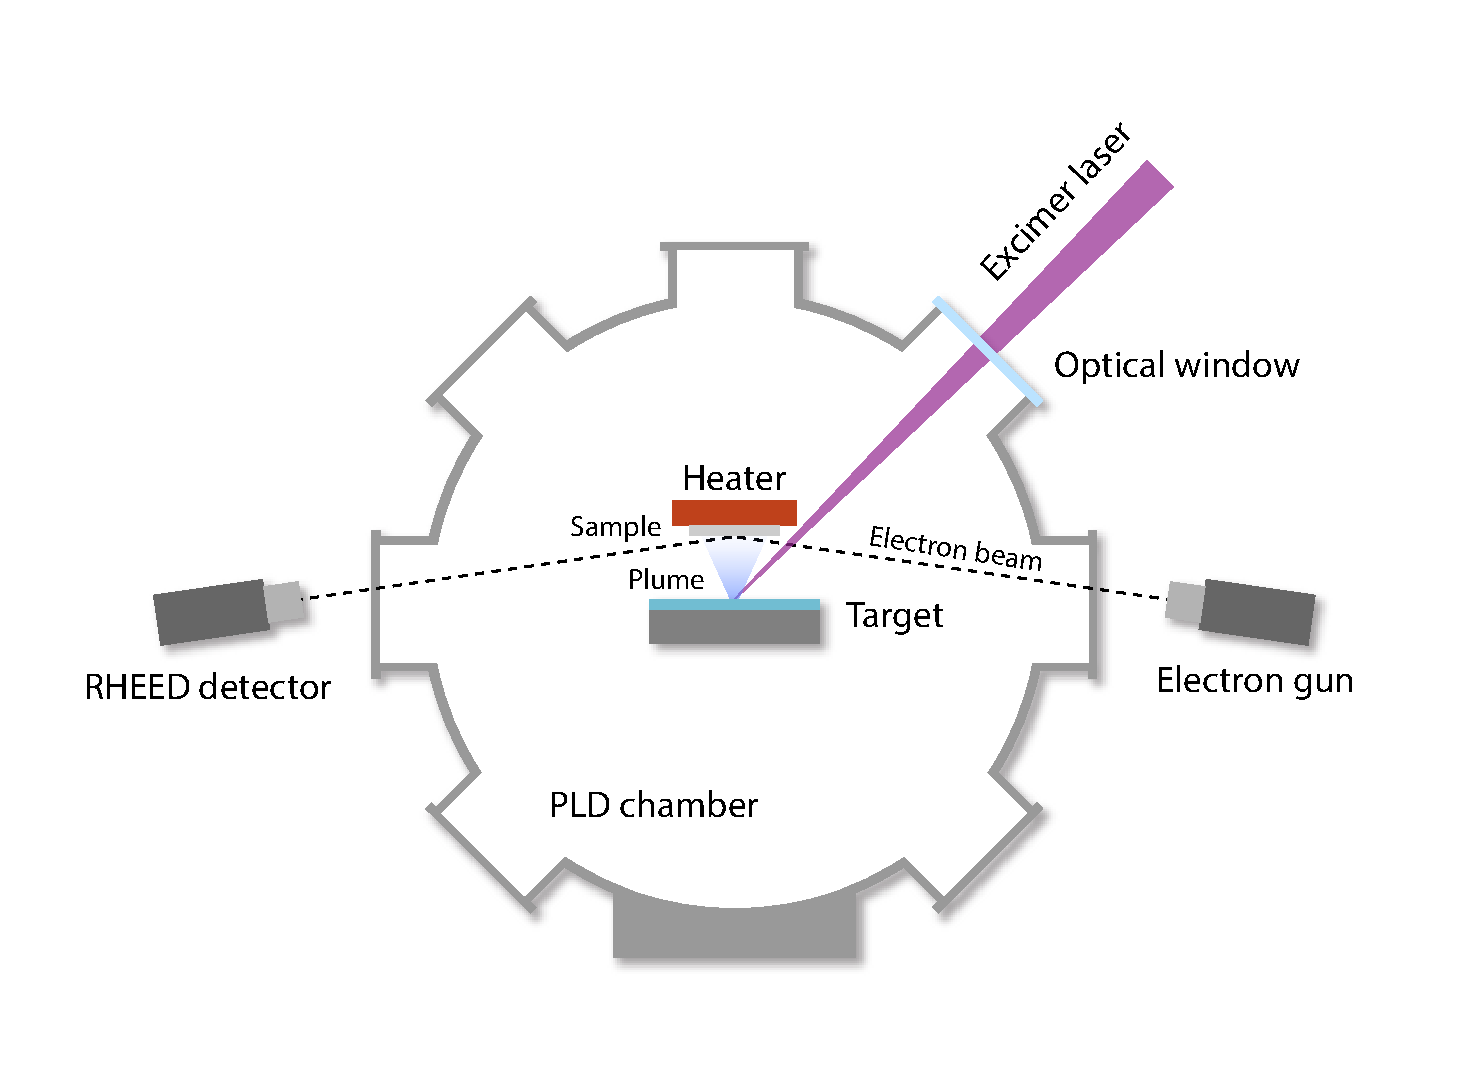
\includegraphics[width=1.0\textwidth]{Drawing/PLD.pdf}
	\caption{PLD epitaxial growth. The PLD chamber is back-filled with oxygen to the target pressure. A beam of pulsed deep-UV excimer laser is focused onto the LAO target. LAO is ablated off and a plume of plasma extends towards the heated substrate on top, and condensed into atomic layer films. RHEED signal is used to monitor the thickness of LAO.}
	\label{FIG:PLD}
\end{figure}

During the PLD growth, the reflection high-energy electron diffraction (RHEED) is used for \emph{in-situ} monitoring the thickness of epitaxial layers. A beam of electron is generated from a source and reflected from the substrate as the film growth. Electron diffraction signal is collected by a detector on the other side (Figure \ref{FIG:RHEED}(a) inset). The intensity of the diffraction oscillates as a function of film thickness. The thickness of LAO can be precisely controlled by counting the cycles of RHEED signal (Figure \ref{FIG:RHEED}(b)).

\begin{figure}[hp!]
	\centering
	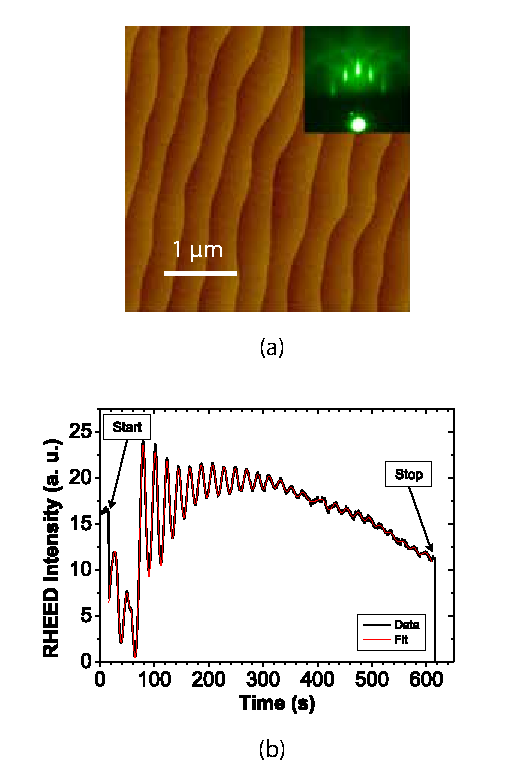
\includegraphics[width=0.7\textwidth]{Drawing/PLD_RHEED.pdf}
	\caption{AFM image of the sample after PLD growth and RHEED signal for PLD. (a) shows is the AFM Image. The stripes are the crystal terraces, with $h \approx 4 \mathrm{\AA}$. Inset of a is the raw diffraction sigal of RHEED. (b) is the RHEED signal oscillation during the film epitaxial growth. Each cycle indicates the completion of one unit cell. Adapted from \cite{podkaminer2016real}.}
	\label{FIG:RHEED}
\end{figure}

% miscut angle and terraces
% figure of PLD
% figure of REED
% figure of AFM (use the 12uc MFM image)
% figure of terraces linecut (use the 12uc MFM image)
% figure of samples with holes

\subsection{Graphene growth}

The two most popular methods to obtain single-layer/few-layer graphene are mechanical exfoliation and chemical vapor deposition (CVD). 

The mechanical exfoliation isolate single layer graphene directly with adhesive tapes. Graphene is a type of Van der Waals material, which means that the carbon atoms within a layer are tightly bonded with covalent bond while the layers are bonded by the much weaker Van der Waals force. Adhesive tapes can easily separate graphene layers. After multiple exfoliation steps, single layer graphene flakes can be separated and identified\cite{}. One key aspect of the exfoliation method is choosing a proper substrate so that single layer graphene can be easily identified with optical microscopes. Although graphene has the highest absorption coefficient in the visible light regime\cite{}, spotting a single layer graphene flake on a transparent substrate is still challenging, and is always assisted with other characterization methods such as Raman spectroscopy\cite{} to ensure the graphene is single layer. The most commonly used substrate is silicon wafer with 400 nm thick silicon oxide coating. The graphene on SiO$_2$ surface modifies the interference of visible light between the top and bottom layer of the coating, and make graphene layers distinguishable\cite{}. 

CVD is another method to obtain single layer graphene. Graphene flake from mechanical exfoliation is mostly a few micrometers or tens of micrometers; the size and shape cannot be well controlled. CVD on the other hand, can grow continuous graphene of wafer sizes\cite{}, and then etch it into any desired shapes through post processing. 

The CVD process uses gaseous organic molecules (methane, ethylene, etc) as carbon source, and graphene lattice-matching crystal such as SiC, Ni and Cu as substrate. In high temperature (about 1000 $^{\circ}$C), the metal surface has highly reactive and can serve as a catalyst, so the gas molecules will react with the surface and carbon atoms are detached. At the high temperature, the carbon atoms will self-assemble into graphene. Over the entire process the substrate is in continuous gas flow so the gaseous byproducts are flushed away. Hydrogen is used to assist the growth. Without hydrogen molecules, graphene will grow simultaneously on the entire surface and form many small domains. Hydrogen will etch away the smaller domains while the larger domains are growing\cite{} until the domains meet or the process is terminated. If the hydrogen portion is too high however, the larger graphene domains will also be etched. CVD is a dynamic process of etching and growth. The ratio of methane and hydrogen need to be carefully controlled.

\begin{figure}[h!]
	\centering
	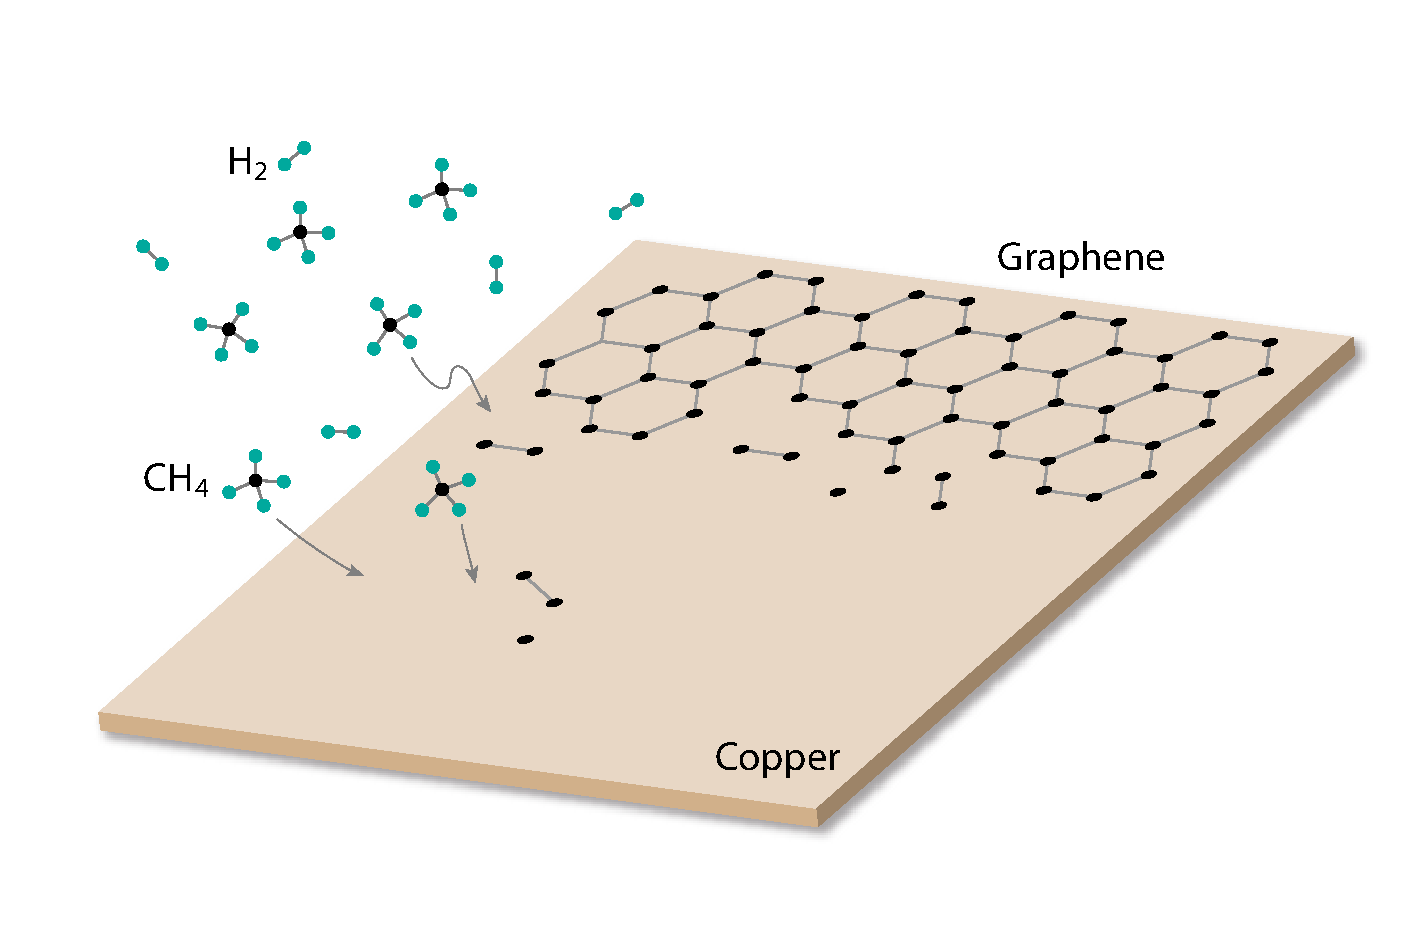
\includegraphics[width=.90\textwidth]{Drawing/CVD.pdf}
	\caption{Graphene CVD growth. At a temperature $T \approx$ 1000 $^{\circ}$C, methane molecules will react with copper surface and leave carbon atom on the surface. Carbon atom will self-assemble into graphene due to lattice-match between graphene and copper super-cell. Hydrogen is used to etch away the smaller domain so that the final single layer graphene domains is as large as possible. If the hydrogen is too much, the larger domain will be etched as well. Ratio of methane and hydrogen has to be carefully controlled.}
	\label{FIG:CVD}
\end{figure}

\subsubsection{Copper substrate preparation}

Various materials are used for graphene growth, most commonly SiC, Ir, Ni and Cu. Cu is the most common choice due to the low carbon solubility scalability\cite{Bae2010}. Compared to other substrate materials, copper is also easy to be etched with wet chemicals. In CVD growth, the carbon atoms form into graphene following the shape of the substrate. Therefore, the graphene quality is directly related to the substrate. Surface roughness and contaminants on copper provide nucleation centers for graphene, and can cause polycrystalline structure and multi-layer growth\cite{eres2014cooperative}. The issue of surface roughness can be addressed with electrochemical polishing\cite{Bae2010}, or mechanical polishing. In my experiment I used a graphene substrates polishing procedure developed by Dr Brian D'Urso's graduate students, by using diamond turning machine to reduce the roughness from several hundred of nanometer to a few nanometers\cite{dhingra2014chemical}. Compared to electrochemically polished substrates, this method can produce surface 50 time smoother and the copper domain sizes are 5 time larger. 

Diamond turning machine (DTM) is commonly used for high precision manufacturing, such as laser reflective mirrors. The DTM works like a lathe, where the workpiece is fixed on a turning spindle, and the cutting tool approaches the workpiece and shape or polish the surface by steps. Figure \ref{FIG:DTM} shows the DTM at work. The cylindrical metal piece in \ref{FIG:DTM}(a) is the spindle of DTM. Copper piece is fixed on the spindle by vacuum and spins at 2000 rpm. The diamond tool approaches the copper surface from the opposite side.  \ref{FIG:DTM}(b) is an image taken in the middle of a cutting step. Mineral spirit is sprayed from a nozzle from the left, cools down the surface and blow away the metal debris to the right. Reflection of the tool shows a flat finishing.

\begin{figure}[h!]
	\centering
	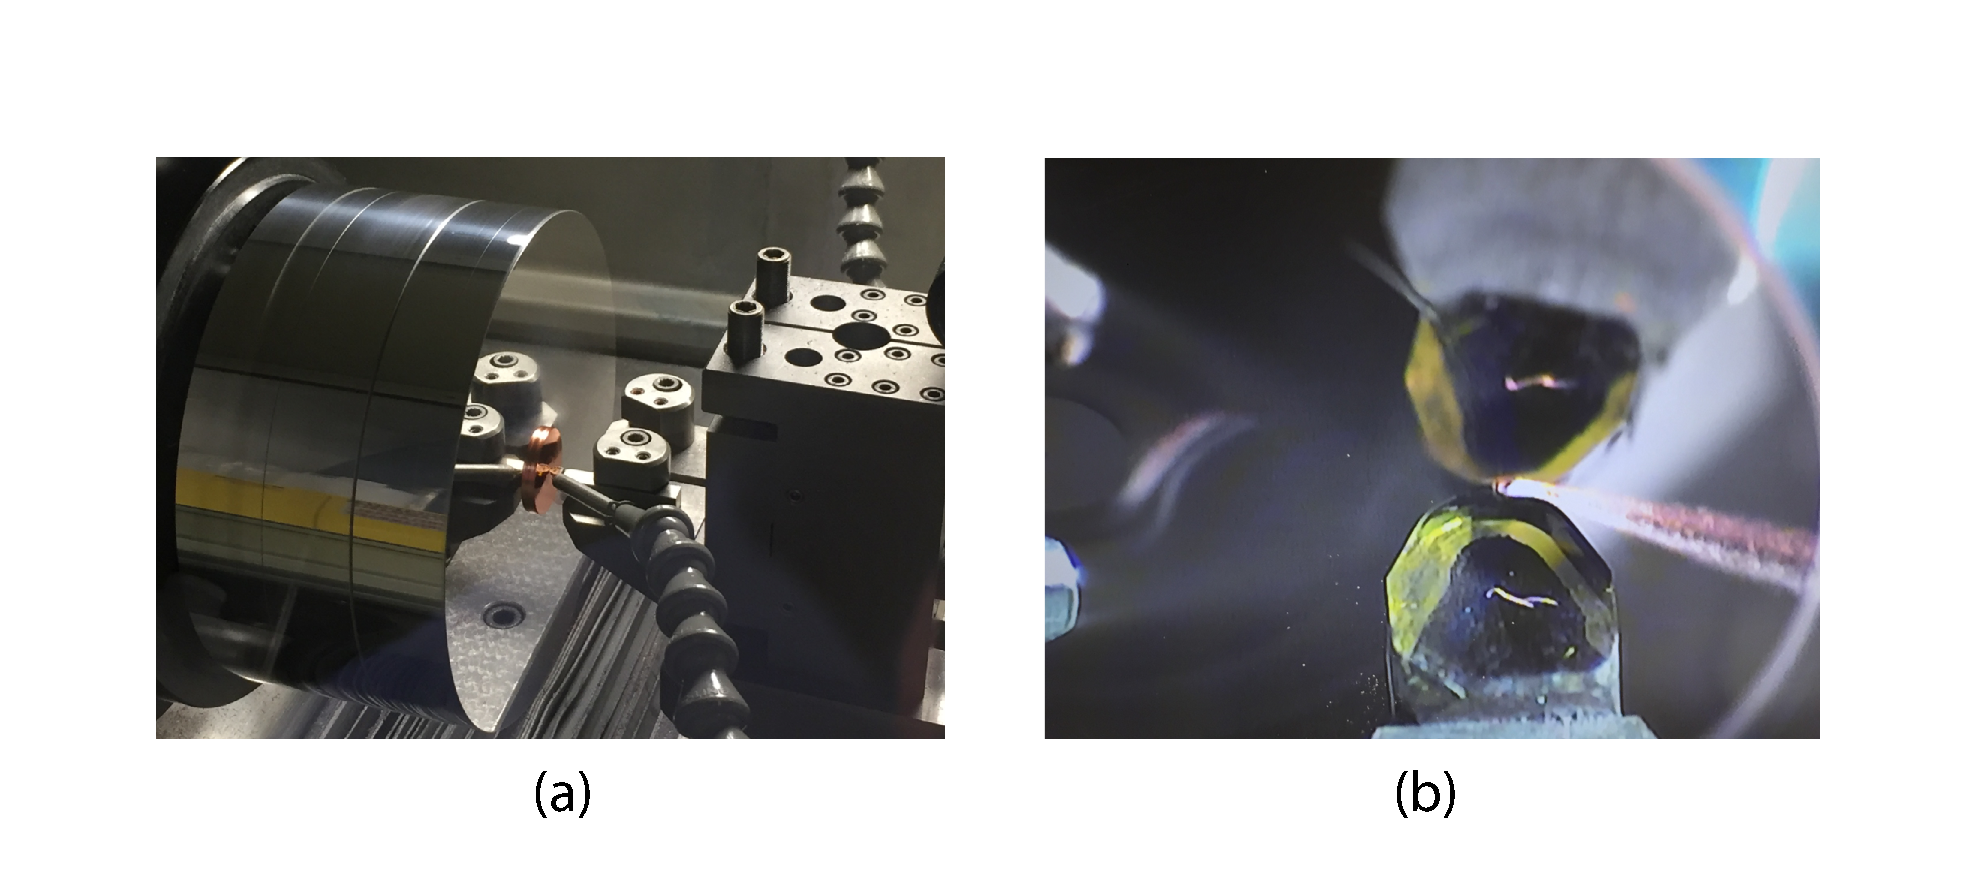
\includegraphics[width=1.0\textwidth]{Drawing/DTM.pdf}
	\caption{Diamond turning machine at work. (a) Copper is fixed onto a turning spindle with vacuum. (b) Mineral spirit is sprayed to the tool and cutting spot, to cool down the surface and blow away the debris.}
	\label{FIG:DTM}
\end{figure}

Instead of using high-speed-steel tool, the DTM uses a curved-edge (radius of curvature $r$ = 1.5 mm) diamond tool for cutting (Figure \ref{FIG:DiamondTool}). By reducing the incremental step to 10 $\mu$m, as shown in Figure \ref{FIG:DTMFinishing}, the roughness of the finishing surface can be smaller than 2 nm. The diamond tool sometimes have dents on the surface, which can leave a trace after each revolution.

\begin{figure}[h!]
	\centering
	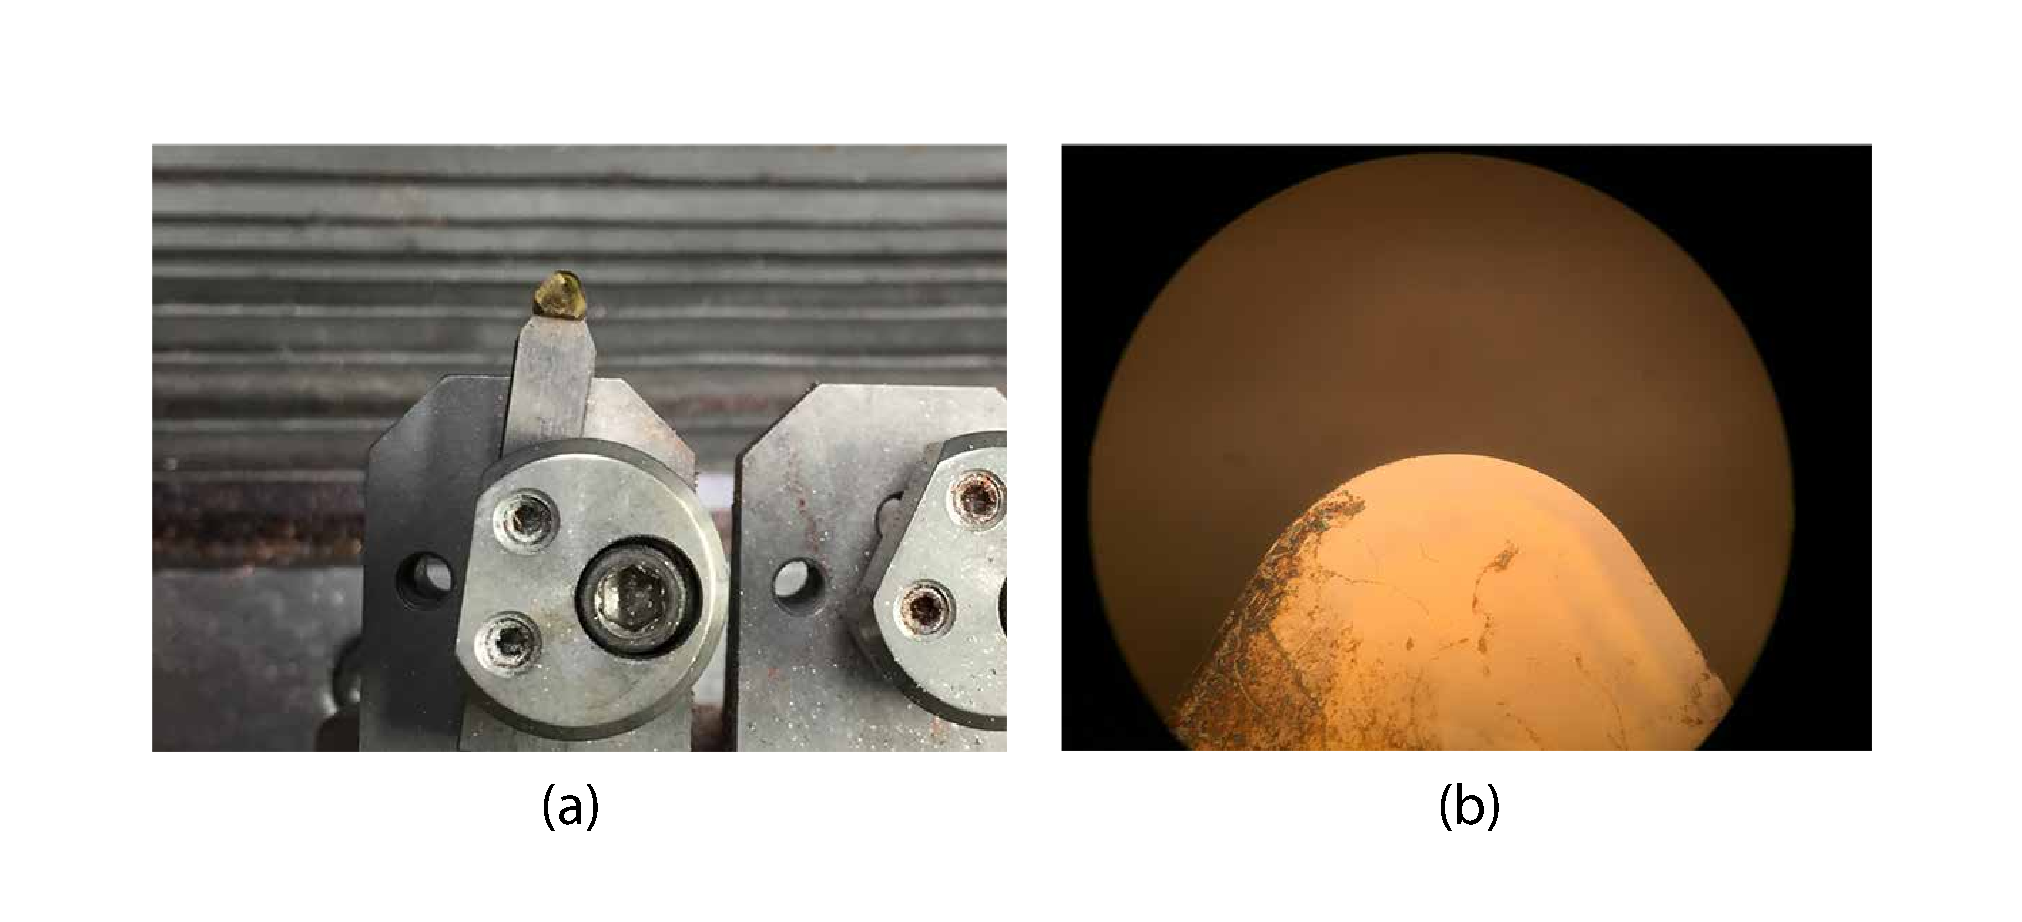
\includegraphics[width=1.0\textwidth]{Drawing/DiamondTool.pdf}
	\caption{(a) Diamond cutting tool. (b) Magnified image of the tool tip. The radius of curvature $r = 1.5$ mm.}
	\label{FIG:DiamondTool}
\end{figure}

\begin{figure}[h!]
	\centering
	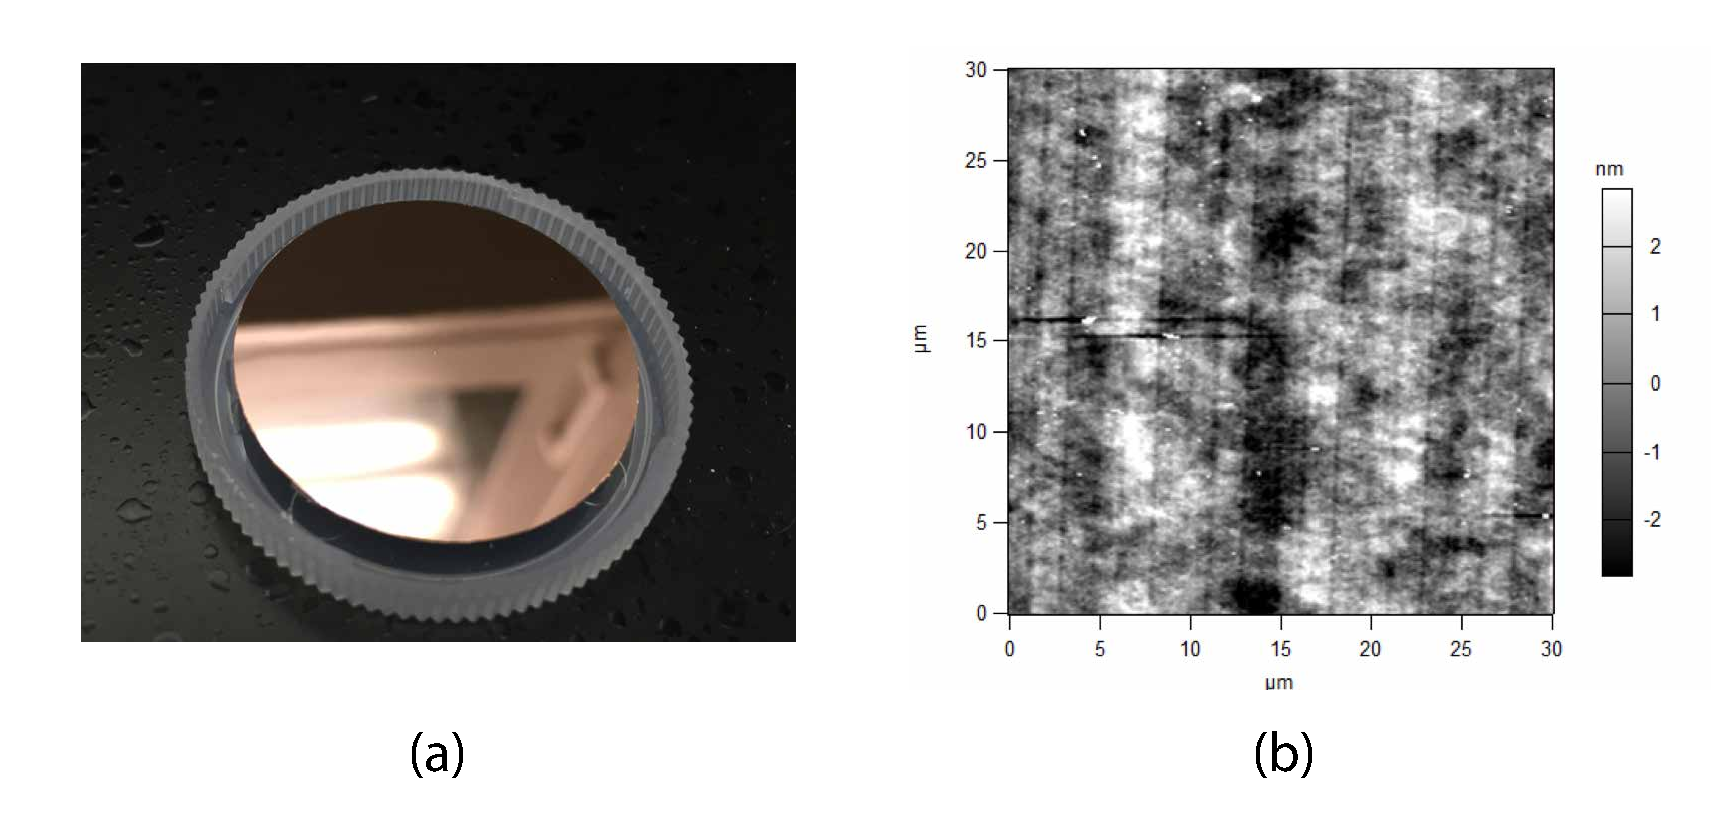
\includegraphics[width=1.0\textwidth]{Drawing/DTMCopper.pdf}
	\caption{(a) The copper foil after DTM thinning and polishing. The final thickness is about 100 $\mu$m. (b) The AFM image of the copper foil surface. The roughness is within 2 nm. Some nanoscale particles can be seen. They will serve as nucleation centers for graphene CVD growth. Reducing the density of surface contaminants will reduce the density of nucleation centers and enlarge the domain size. The vertical groves are left by the dents on the diamond tool for each revolution. The spacing between groves is the same as the approaching speed of the tool towards the center. The copper is annealed at $T = 1050^{\circ}$C for another time before growth starts and the surface will reconstruct, possibly remove those groves.}
	\label{FIG:DTMFinishing}
\end{figure}

Other than surface roughness, the copper domain size is another limiting factor for large single domain graphene growth. Although it was not clear the effect of copper substrate domains on the graphene quality\cite{kim2012direct, wang2012controllable, wofford2010graphene}, larger copper domain sizes gives us a chance to grow larger graphene single crystals. Annealing the copper at high temperature will reconstruct and merge the polycrystalline domains into larger domains, but mechanical processing will introduce defects and break the single domains, therefore the substrate needs to be re-annealed several times before graphene growth starts.

\begin{figure}[p]
	\centering
	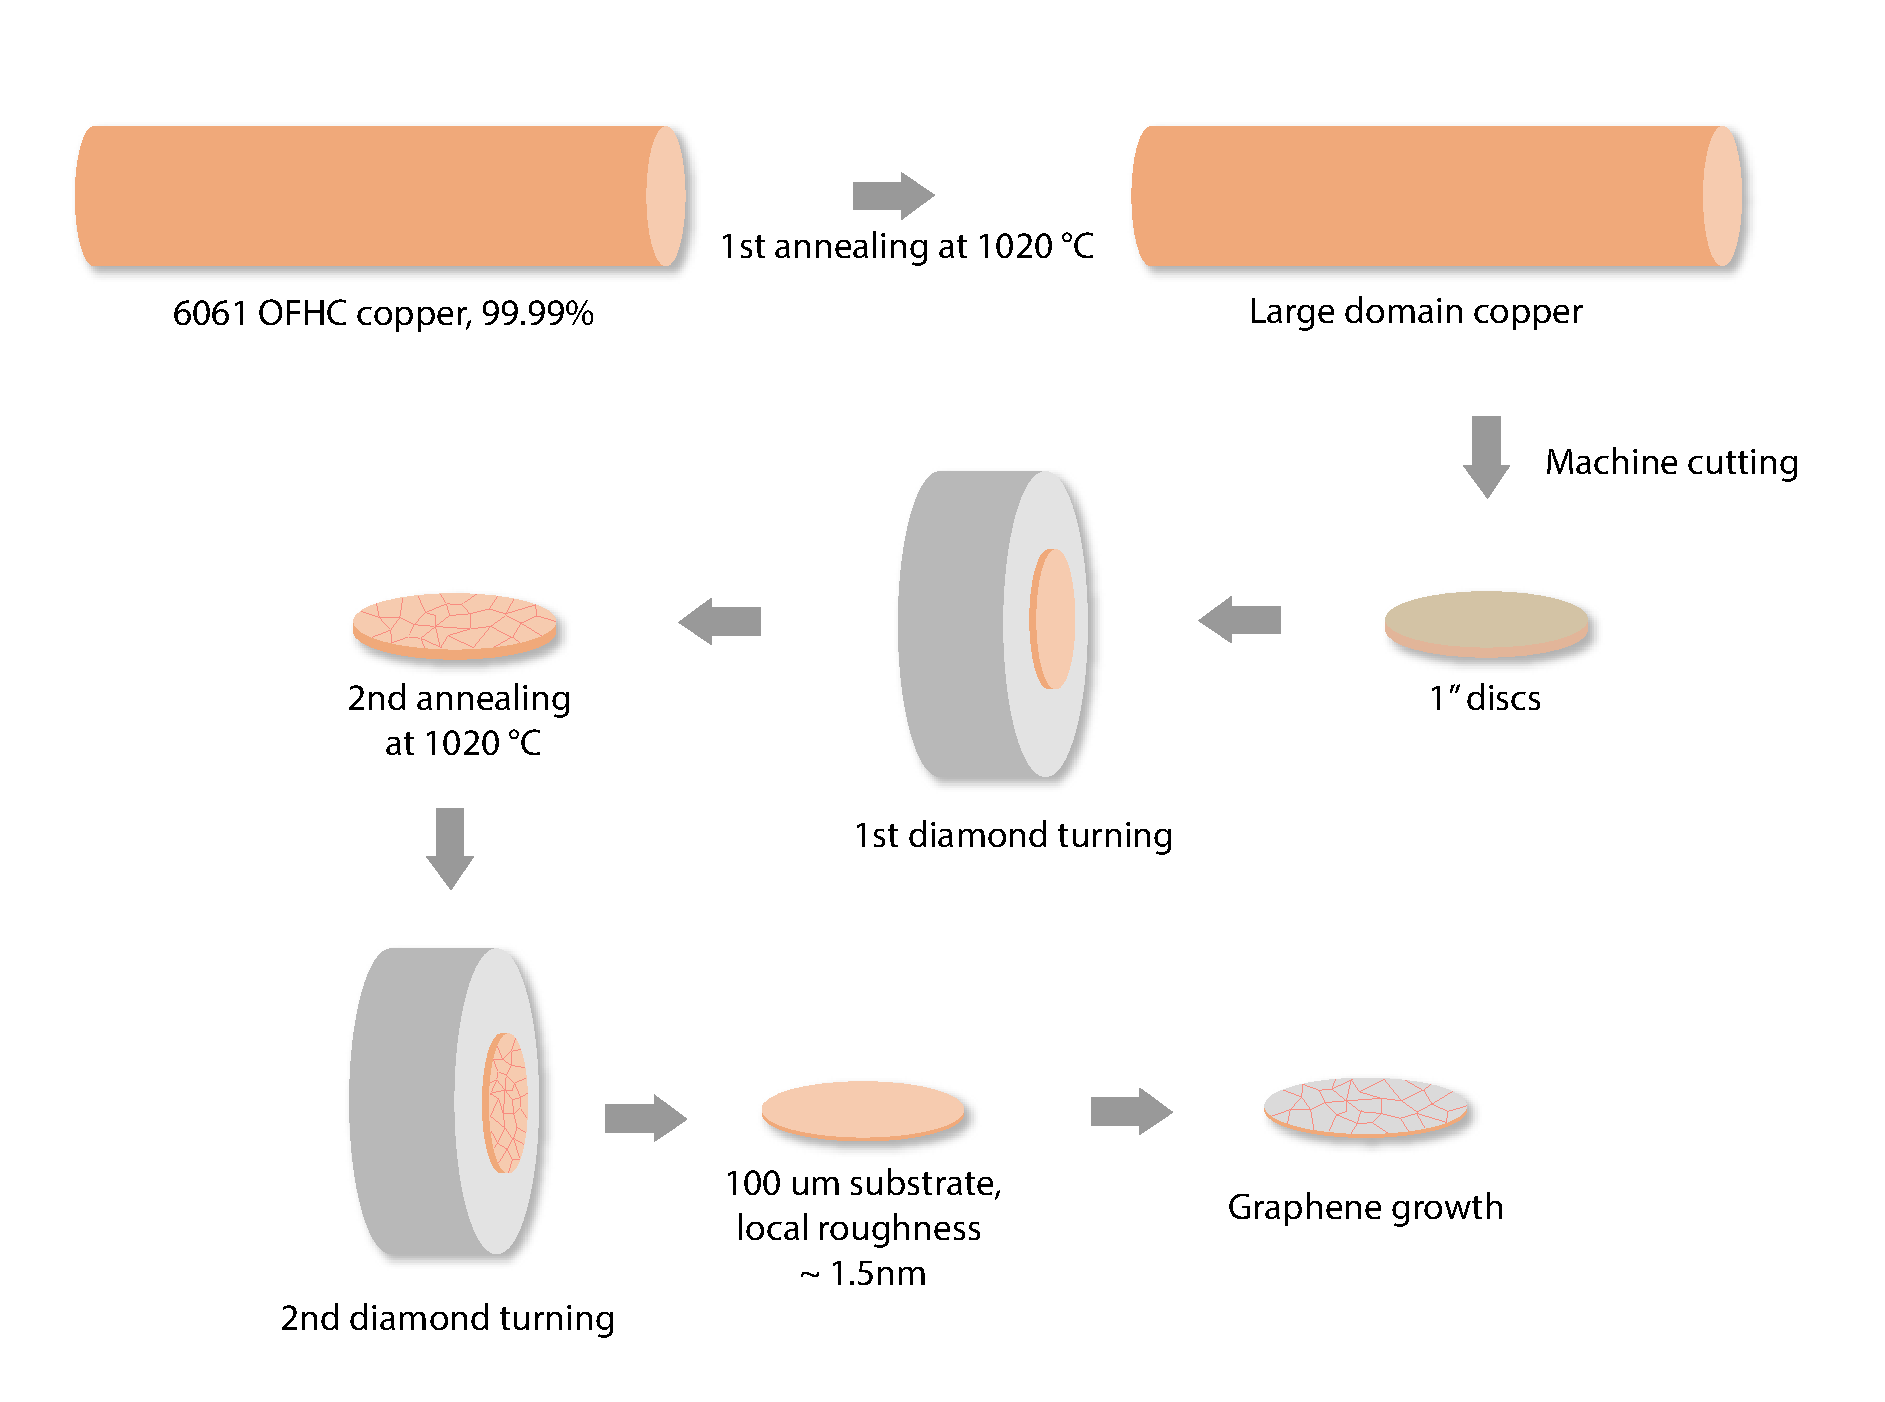
\includegraphics[width=1\textwidth]{Drawing/CopperProcessing.pdf}
	\caption{Procedure of cutting copper rods into 100$\mu$m foils for graphene growth. High purity OFHC copper rods are purchased from McMaster Carr. The rod is first annealed at 1050$^{\circ}$C for 24 h so that the polycrystalline domains merge into larger domains. Then the rod is cut into 2 mm thick copper discs in the machine shop. The discs are cleaned with DTM and then annealed again to ``heal'' the domains broken by the mechanical cutting. Domain re-formation would cause surface corrugation, therefore the copper disc surface is cleaned with DTM and then cut into 100 $\mu$m foils and ready for graphene CVD growth. }
	\label{FIG:CopperProcessing}
\end{figure}

The procedure of making copper rods into copper foils for graphene growth in shown in Figure \ref{FIG:CopperProcessing}. 1' long oxygen-free high thermal conductivity copper (OFHC) rods with ultra high purity (99.99\%) are purchased form McMaster Carr. The rod is first annealed at $T=1050^{\circ}$C for 24 h, and the polycrystalline domains will merge into larger domains within the rod. Then the rod is cut into copper discs of 2 mm thick in the machine shop. The mechanical cutting process will break the domains and introduce surface contaminant, so the surfaces copper discs are cleaned on the DTM, and then annealed again at 1050 $^{\circ}$C for 8 h. After annealing, the domain re-formation in the disc will cause corrugation on the surface. Therefore, the copper surface is cut with DTM for a second time. Then the copper discs are cut into 100 $\mu$m foils, by 10$\mu$m steps. During the thinning procedure, the copper will expand on the cutting face and cause deformation, and eventually break the vacuum sealing between the disc and spindle on the backside. Therefore the copper disc needs to be flipped several times to balance out the expansion and keep it flat when thinned from 2 mm to 100 $\mu$m. The process takes about 5 h. 

\subsubsection{CVD growth}

The CVD graphene growth can be performed in low pressure (LPCVD) or atmospheric pressure (APCVD). LPCVD grows graphene at a pressure lower than 100 mTorr, in continuous flow of pure hydrogen and methane and 1000 $^{\circ}$C substrate temperature. The problem with LPCVD is that the melting point of copper ($T_m = 1085^{\circ}$C) is close to the growth temperature. As a result, the copper will evaporate severely and contaminate the furnace\cite{vlassiouk2013large}. Also the pure precursor gases bring fire hazard. APCVD can eliminate those difficulties associated with the low pressure and improve the graphene quality\cite{vlassiouk2013large, dhingra2015quadratic}. Instead of using pure hydrogen and methane, APCVD uses gas mixture of 2.5 vol \% H$_2$, balance Ar and 0.1 vol \% CH$_4$, balance Ar. The furnace is pumped into low vacuum, and then backed-filled with hydrogen and methane mixture with argon to atmospheric pressure. The pressure from argon will suppress the evaporation of copper at annealing and growth temperature. The growth procedure are as follows\cite{dhingra2015quadratic}. 

\begin{itemize}
	\item The furnace is pumped down to $\sim$ 10 mTorr.
	\item Backfill the furnace with H$_2$/Ar mixture at 186 sccm, up to $\sim$ 100 Torr.
	\item Start the furnace temperature controller to ramp up to $T = 1050 ^{\circ}$C, and let the furnace stay at this temperature for 1 h.
	\item Start flowing mixture of CH$_4$/Ar at 14 sccm into the furnace, and let the copper foil stay in graphene CVD growth condition for 1.5 h.
	\item Cool down the system to room temperature. The flow of CH$_4$/Ar mixture is turned off at $\sim$ 650$^{\circ}$C. H$_2$/Ar mixture keeps flowing overnight until the system is below 50$^{\circ}$C. 
	
\end{itemize}

\begin{figure}[p]
	\centering
	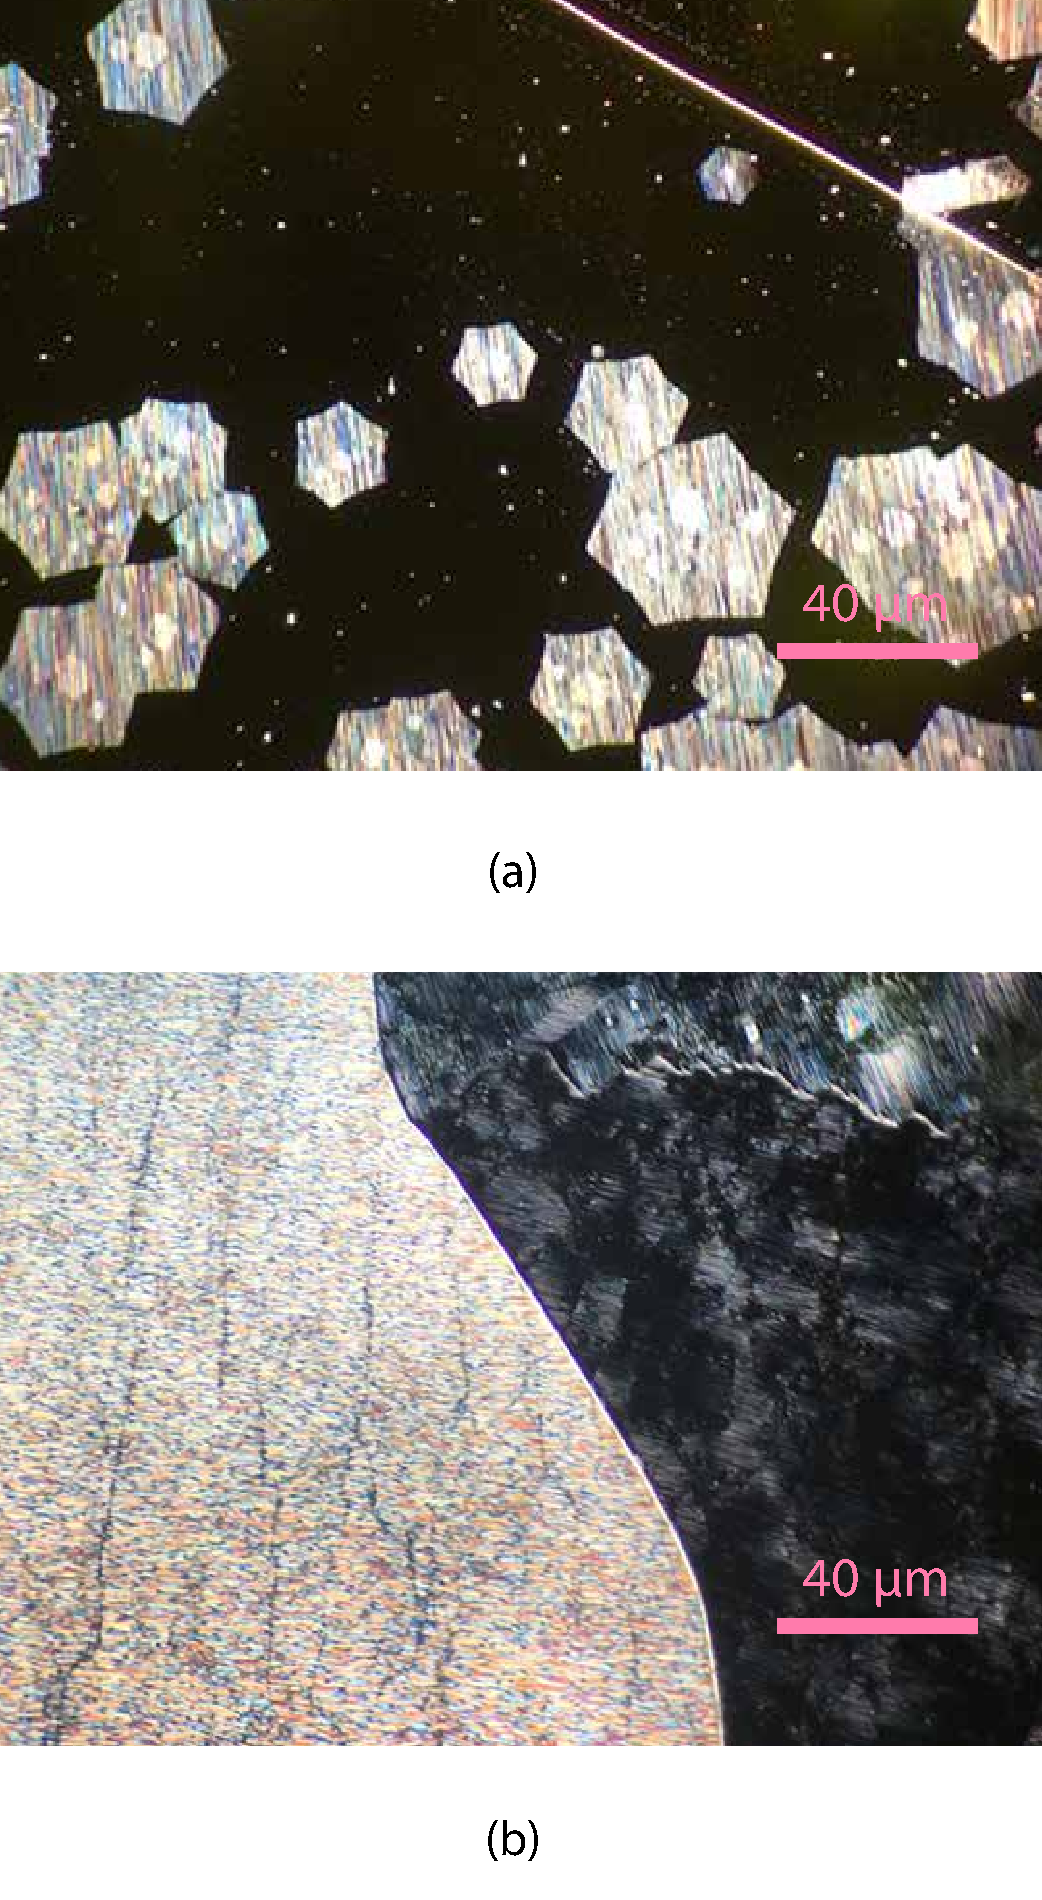
\includegraphics[width=0.6\textwidth]{Drawing/CVDGraphene.pdf}
	\caption{Dark field mode microscope images of CVD graphene on copper substrates. (a) The copper substrate is partially covered with graphene. Hexagonal shape single domain graphene can be observed. Growth was terminated before graphene fully covered the substrate. (b) Graphene covers the entire copper substrate. Copper domains of two different orientations can be observed. }
	\label{FIG:CVDGraphene}
\end{figure}

In Figure \ref{FIG:CVDGraphene} the dark-field mode of optical microscope clearly shows the CVD graphene on copper substrates. In \ref{FIG:CVDGraphene}(a) the copper substrate is partially covered with graphene. Growth process was terminated before graphene fully covered the substrate. Hexagonal shape of single domain graphene flakes can be identified. Some double layer can also be observed. On the top right corner of \ref{FIG:CVDGraphene}(a) a copper domain boundary can also be identified. \ref{FIG:CVDGraphene}(b) is the image of graphene grown in another run. The substrate is fully covered with graphene. The image shows two copper domains with different orientations, and therefore the graphene grown on the two domains look different. Wrinkles on graphene can be observed, resulting from different thermal expansion coefficient of copper and graphene. 

\section{LAO/STO sample processing}

One of the challenges with experiments on LAO/STO interface is to make good electrical contact from the bonding pads to the interface. A major part of my research is process the samples before the c-AFM writing can be performed, or graphene can be transferred. The processing methods have to be carefully chosen, so that the 2DEG and interface switchability will not be affected. Sample cleanness is another concern. Any nano-particles introduced in the processing would affect sample quality, considering that the dimensions of devices are also nanoscale. The procedure has those steps. Details of each steps can be found in the following subsections.

\begin{itemize}
	
	\item \textbf{Initial cleaning}: the sample is cleaned with acetone and isopropanol alcohol (IPA) in ultrasonic cleaner so that the particles introduced in shipping are cleaned. Usually we do not use deionized-water (DI-water) for cleaning. Proton from the water can get adsorbed on sample surface and affect the interface \cite{}.
	
	\item \textbf{Photolithography}: the sample is patterned with standard UV photolithography procedures, either with optical mask and UV lamp or with direct laser writer, for further processing. The finest features in my design are 2 $\mathrm{\mu}$m wide.
	
	\item \textbf{Ion milling}: after the desired patterns are developed on the photoresist, the sample is bombarded with Ar$^+$ ion flow so that the LAO/STO interface is exposed for electrical contact.
	
	\item \textbf{Deposition}: titanium and gold are used for making contact with the exposed LAO/STO interface either by electron-beam evaporation or sputtering.
	
	\item \textbf{Lift-off}: the excessive metal outside the patterns are removed by the lift-off process following the metal deposition. Like the initial cleaning process, we use IPA and acetone and do not use water as solvent.
	
	\item \textbf{Oxygen plasma cleaning}: the sample is covered with residue from liquid and photoresist, until it is cleaned with oxygen plasma cleaner. Then the atomic steps can be seen with AFM.
	
\end{itemize}
	
The sample processing procedures are shown in FIG. \ref{}. 

% figure of processing

\subsection{Photolithography}

Photolithography is a commonly used technology in semiconductor industry. The substrate is covered with a thin layer of photosensitive material, and exposed under UV with designed pattern. UV would change the solubility of photoresist, and the pattern can be developed in buttered base solution after exposure. The modern state-of-the-art photolithography technology can reach resolution of 10 nm, and is the pillar of support for the semiconductor industry. There are two types of photoresists: positive and negative. Positive photoresist will be washed off after been exposed to UV, while negative photoresist is stabilized by UV and the unexposed parts are removed by developers. In my experiment, three types of positive photoresists are used: AZ4620, AZ4210 and AZ4110. For each sample, a 3'' carrier wafer is used as a fixture, because dimensions of the sample (5 mm $\times$ 5 mm $\times$ 1 mm) is non-standard and most photolithography instruments are designed for 3'' or 4'' wafer in the university facility. AZ4620 is used to fix the sample to the carrier wafer during spin-coating, exposure and other steps, as a cleanroom-safe ``epoxy''. 


\subsubsection{Spin-coating}

There are two limiting factors of the feature resolutions in photolithography: diffraction limit of light and photoresist thickness. Spin-coating is a standard technique to keep the photoresist thin and uniformly covering the sample surface. When the sample is spinning at a speed between 1000 rpm and 6000 rpm, the photoresist solution on sample surface would spread out. The liquid will be finally in equilibrium of viscosity, roughness of sample surface and centrifugation from spinning. After the spin-coating the sample is baked at a temperature around 100$^{\circ}$C to vaporize the remaining solvent in photoresist and stabilize the film befor UV exposure. In my experiment, the spinning speed is 4000 rpm. Thickness of AZ4210 and AZ4110 are 2.1 $\mu$m and 1.1 $\mu$m, respectively. These two types of photoresists have the same chemical composition. They have different concentrations so they end up with different thickness at the same speed. Usually thinner films will have more stable performances for fine features (2 $\mu$m, to be specific). In the cases where photoresists are consumed in the processing, such as reactive ion etching, thicker photoresist will be a better option.

The spin-coating conditions are listed in Table \ref{tab:photoresistsCoating}.

\begin{table}
	\centering
	\begin{tabular}{l|cc}
		\hline
		Photoresist	&	AZ4210	&	AZ4110 \\ \hline
		Spinning speed	&	4000 rpm	& 4000 rpm	\\ 
		Spinning time	&	30 s	&	30 s	\\
		Baking temperature	&	95 $^{\circ}$C	&	95 $^{\circ}$C \\ 
		Baking time	&	60 s	&	60 s	\\
		Thickness	&	2.1 $\mu$m	&	1.1 $\mu$m \\ \hline
	\end{tabular}
	\caption{Spin-coating conditions for AZ4210 and AZ4110}
	\label{tab:photoresistsCoating}

\end{table}

% image of sample spin coated with photoresist. Explain the color stripes.

\subsubsection{UV exposure}

The UV exposure is to use short wavelength photon to change the solubility of photoresist, so that the following developing step can selectively remove the photoresist. Like all optical system, the resolution of exposure is limited by diffraction limit of light. Historically, mercury gas-discharge lamp is used, and 436 nm (``g-line''), 405 nm (``'h-line') and 365 nm (``i-line'') are selected as UV source. Besides Hg lamp, solid state laser and excimer laser with shorter wavelengths are also commonly used UV source. Samples are exposed with two different methods: mask exposure and direct laser writing. 

Mask exposure is performed by a mask aligner (Suss MJB3 or MA6, see Figure \ref{FIG:Suss}). Incoherent and collimated UV is generated from a Hg lamp and an area of 4'' $\times$ 4'' is exposed with UV at constant intensity of 10 mW/cm$^2$. The sample is covered with a photomask (Figure \ref{FIG:MASK}), a square piece of soda glass (to reduce UV absorption) coated with chromium on one side. The desired pattern is pre-printed on the chromium by chemical etching. The patterns on photoresist will be the copy of the patterns on the photomask. 

\begin{figure}[h!]
	\centering
	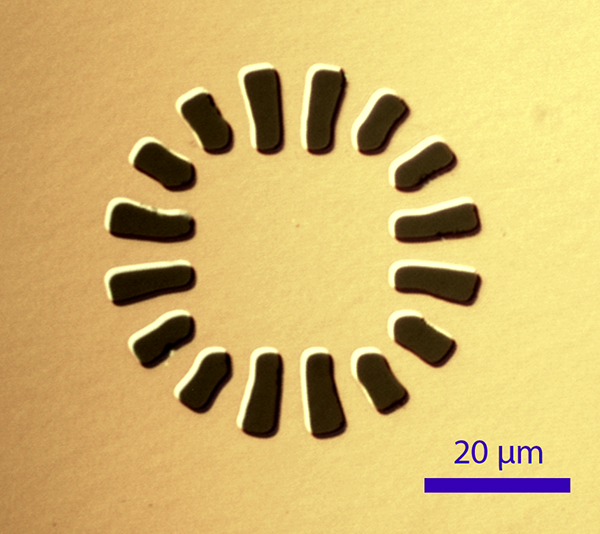
\includegraphics[width=0.5\textwidth]{Drawing/MASK.png}
	\caption{Mask for photolithography. The dark parts are transparant, while the bright parts are covered with chromium. Sample will be exposed where UV is not blocked by chromium. The figure shows the electrodes of a canvas for writing. The pedal shape area to be exposed will be etched away on the sample, and filled with titanium and gold to make contact with the LAO/STO interface.}
	\label{FIG:MASK}
\end{figure}

\begin{figure}[hp!]
	\centering
	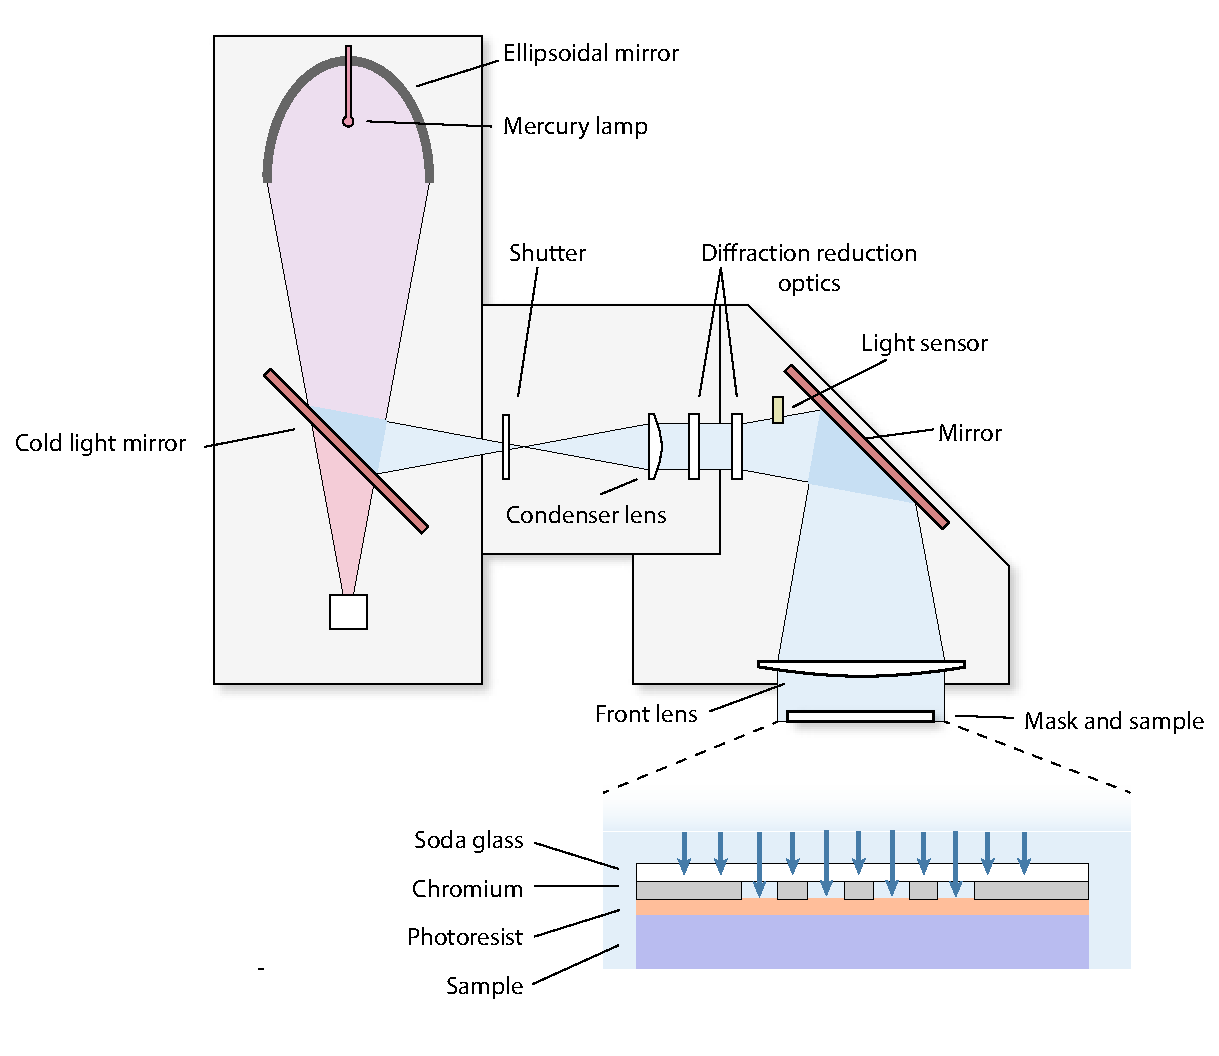
\includegraphics[width=1.0\textwidth]{Drawing/Suss.pdf}
	\caption{Suss UV mask aligner. The mercury lamp generates broad band light from arc. The light is reflected by an ellipsoidal mirror and focused on a cold light mirror, where the UV is selected. The exposure time and dose is controlled by a shutter. The UV is collected by a condenser lens and diffraction reduction optics for collimation and resolution enhancement. Finally, the UV is shed on the sample with a folding mirror and front lens. The sample is in close contact with a mask, where chromium is partially removed. UV exposes the photoresist on sample and print the mask pattern on it.}
	\label{FIG:Suss}
\end{figure}

Direct laser writing uses focused laser beam to write micro-patterns directly on photoresist, without using a mask. This is usually how the photomask is manufactured, but it can also be used to pattern samples. In my experiment I use Heidelberg MLA100 (Figure \ref{FIG:Heidelberg}), with 405 nm wavelength UV generated from a solid state laser. The laser is expanded and filtered with a pinhole, and focused on the sample with a high-NA objective. The focusing objective is fixed, and the sample is placed on a piezostage controlled with computer, to follow the designed pattern. The UV dose is determined by both the laser power and laser spot dwell time. It is important to keep the sample surface horizontal, so that laser spot will not defocus while moving through the entire sample surface. Sometimes, especially when the critical dimension is close to 2 $\mu$m, the photoresist patterns are not evenly developed, and it is caused by sample tilting and laser defocussing. Focusing quality can be checked with a real-time CCD image, while the sample is illuminated with red light from a second diode.

\begin{figure}[hp]
	\centering
	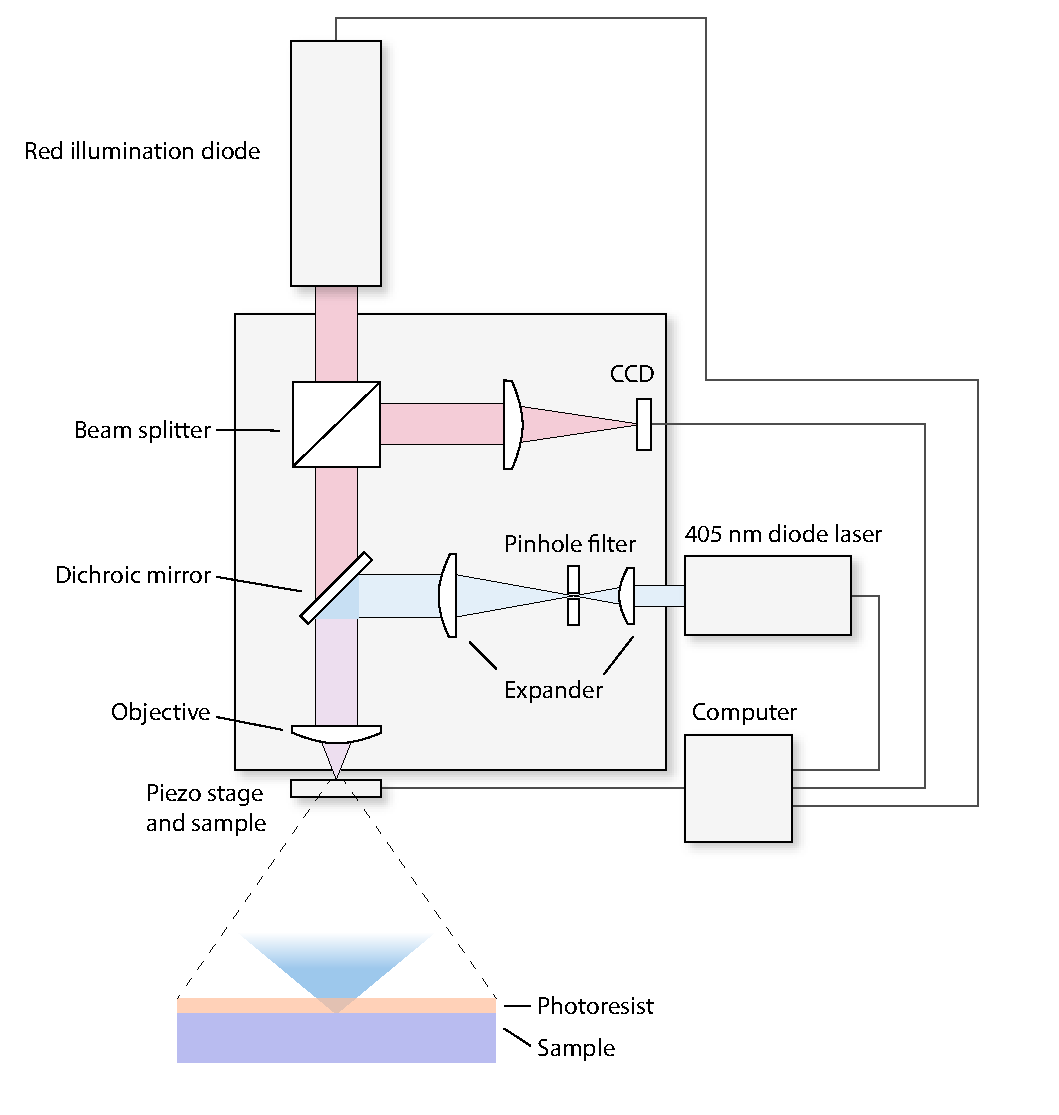
\includegraphics[width=1.0\textwidth]{Drawing/Heidelberg.pdf}
	\caption{Heidelberg direct laser writer. The sample is illuminated by red light from a diode, and realtime image of sample surface can be monitored with a CCD. UV with $\lambda=405$ nm is generated from a laser diode. The laser is expanded and filtered, and focused on the sample surface with a high-NA objective. The sample is fixed on a piezo-driven stage. The CCD image, laser power, sample movement and layer alignment are all controlled with computer, so that the laser path and dose control is fully automatic.}
	\label{FIG:Heidelberg}
\end{figure}

\subsubsection{Developing}

Developing is the process using buffered base solution to washed away the unwanted parts of photoresist after exposure and reveal the pattern on sample, for future processing steps. Depending on the type of photoresist, either the exposed parts (positive photoresist, such as AZ4210) or unexposed parts (negative photoresist, such as AZ5214) are removed. In my experiment I use AZ400K (potassium borate) for developing. The developer is diluted with DI-water, by 1:3 or 1:4 ratio. Different concentration will maintain different pH level and developing speed. The sample is washed with DI-water after developing, to remove the excessive developer. 

A picture of sample after UV exposure and developing is shown in Figure \ref{FIG:Developed}. Photoresist in the bright area are washed away while the rest of the sample is still covered with photoresist. Note that the edges of the pattern are less sharp than the mask, because of the resolution limit from diffraction. 
\\
\begin{figure}[h!]
	\centering
	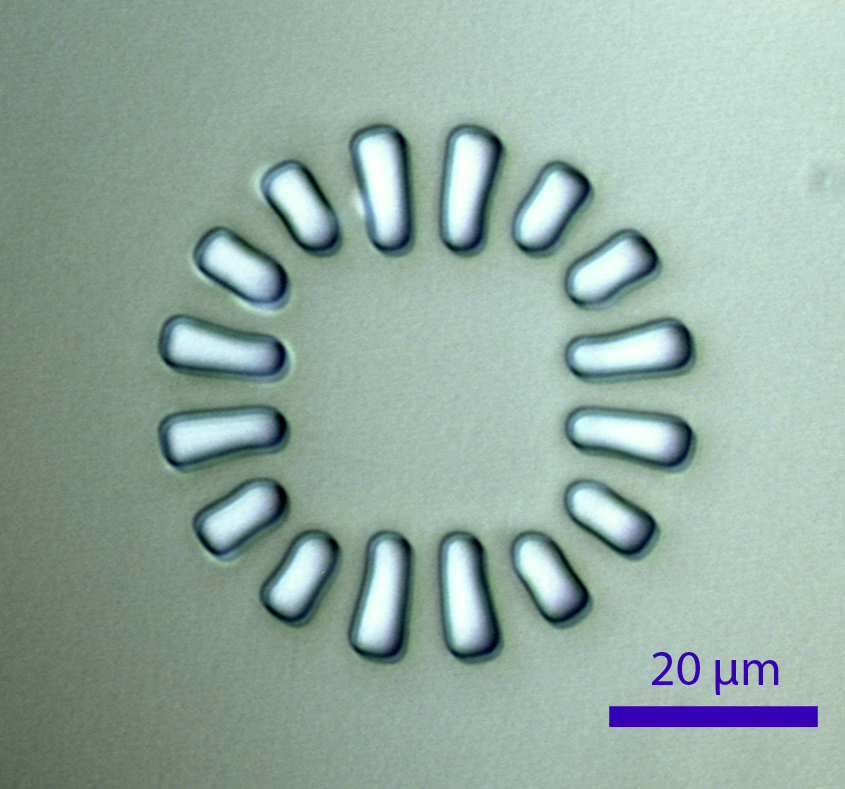
\includegraphics[width=0.5\textwidth]{Drawing/Developed.png}
	\caption{Exposed and developed sample. The bright regions are free of photoresist while the rest of the sample is still covered.}
	\label{FIG:Developed}
\end{figure}

The conditions for exposure and developing are listed in Table \ref{tab:photoresistsExposureDeveloping}.

\begin{table}[h!]
	\centering
	\begin{tabular}{l|cc}
		\hline
		Photoresist	&	AZ4210	&	AZ4110 \\ \hline
		UV Dose	&	170 m$J$	& 100 - 120 m$J$	\\ 
		Developer : Water	&	1 : 4	&	1 : 4	\\
		Developing time	&	120 - 180 s	&	120 - 180 s \\ 
		Resolution	&	3 - 5 $\mu$m	&	2 $\mu$m	\\ \hline
	\end{tabular}
	\caption{UV exposure and developing conditions for AZ4210 and AZ4110}
	\label{tab:photoresistsExposureDeveloping}
	
\end{table}

 Photolithography is the part that has the most uncertainty in the entire processing, and can affect some samples (like graphene/LAO/STO) more significantly. This will be discussed in future sections. 

\subsection{Ion milling}
\label{SEC:IonMilling}
LAO/STO interface is buried underneath LAO, so if contact need to make with the interface the LAO has to be etched. Usually there are three methods for etching: wet chemical etching, dry plasma etching and ion milling. Wet chemical etching using reactive chemical solutions (such as HF, HCl) to etch away the materials. This is  cheaper but less controlled, and etching is isotropic. Plasma etching, uses the plasma or free radicals of active gas molecules (such as O$_2$, SF$_6$, etc) to react and remove materials, at pressure between 0.1 and 5 Torr. It is better controlled in etching rate and directionality, but the instrument is more expensive, and finding the right gas to selectively etch the target material while keeping the protecting layer intact is not always feasible. Although there are mature industrial solutions for silicon, alumina and silica etching with plasma, there is not a good solution to etch complex oxides like LAO/STO with our facility plasma etcher. Ion mill uses accelerated ionized argon plasma to physically bombard sample. The etching rate is slower than the previous two methods, but performs well on most inorganic materials including LAO/STO. Also, the etching is more directional. In Table \ref{tab:etching} is a comparison of the three etching methods.

\begin{table}
	\centering
	\begin{tabular}{l|ccc}
		\hline
		Method	&	Chemical etching	&	Plasma etching	& Ion milling \\ \hline
		Cost	&	low	& high	& high \\ 
		Directionality	&	anisotropic	&	anisotropic	&	isotropic \\ 
		Selectivity	&	high	&	high	&	low \\
		Speed control	&	poor	&	good	&	good \\
		Target material	&	inorganic	&	organic or inorganic	&	inorganic \\
		Environment	&	aqueous, ambient	&	0.1 - 5 Torr, vacuum	&	$< 10^{-4}$ Torr, vacuum \\
		\hline  
		
	\end{tabular}
	\caption{Comparison of etching methods.}
	\label{tab:etching}
	
\end{table}

Ion mill accelerates Ar ions to a certain kinetic energy and physically etch samples with bombardment. As shown in Figure \ref{FIG:IonMill}, Ar$^+$ is generated from the discharge chamber. The entire chamber is pumped to high vacuum ($< 10^{-6}$ Torr), and back filled with Ar gas to $10^-4$ Torr. On the right-hand-side of the figure, a filament is heated up and a biased voltage is applied between the filament and chamber wall. Electrons are extracted from the filament and ionize the argon molecules. Usually a magnetic field is applied through a solenoid to increase the path and ion yield before the electrons reach the chamber wall. At the opening side of the discharge chamber, there are two or three layers of electrically isolated screen grids (made of sputter-resisting materials like Mo or W). A voltage of 500eV is applied between the grids so that Ar$^+$ can be accelerated to the same energy. The pores on the grids are aligned so that the Ar$^{+}$ flow is collimated. Right after the Ar$^{+}$ exits the chamber, it is mixed with free electrons from a neutralizer filament, so that flow will not be diverged by coulomb attraction between Ar$^{+}$ before they reach the sample. The sample is 20$^{\circ}$ to 30$^{\circ}$ off the normal direction, to create undercut and facilitate electrical contact between the interface and the electrodes. The kinetic energy of the plasma is converted to heat on the sample surface. Either the sample is cooled down with flowing water inside the chuck, or the plasma flow is shutoff with a duty cycle so that the sample can cool down by radiation. Temperature over 150 $^{\circ}$C will cause phase transition of the photoresist on the sample, and make hard to remove by lift-off.

\begin{figure}[hp]
	\centering
	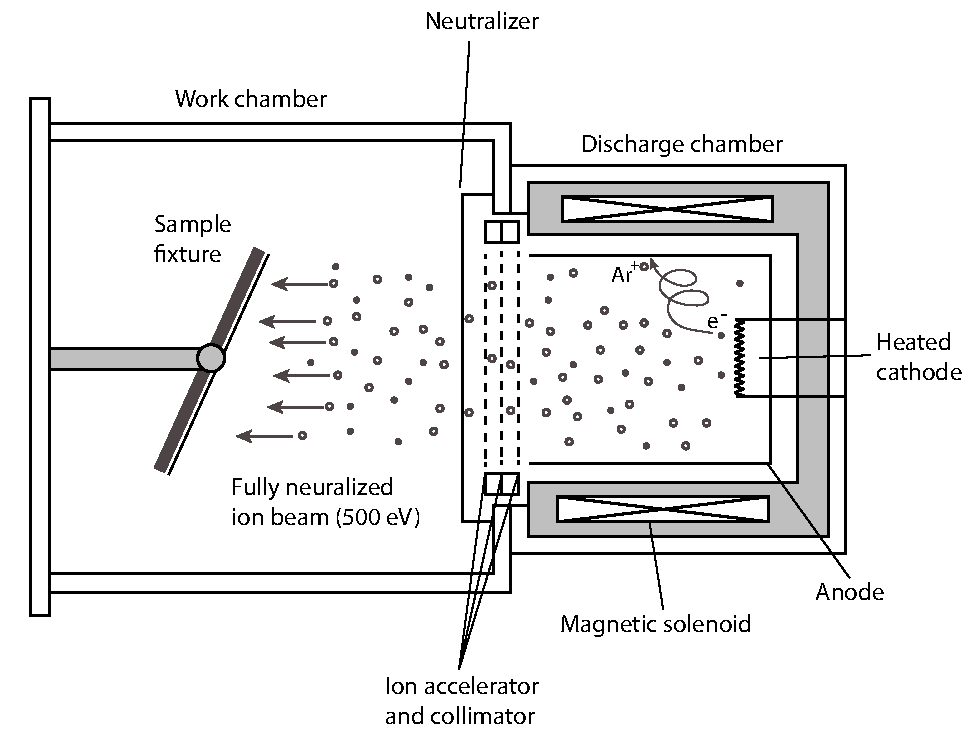
\includegraphics[width=1.0\textwidth]{Drawing/IonMill.pdf}
	\caption{Simplified view of ion mill. The argon ions are generated from the discharge chamber on the right hand side. Electrons are extracted from the heated cathode and ionize Ar molecules before they reach the chamber, which works as an anode cup. A magnetic field is applied through a solenoid to increase electrons' path. Ar$^{+}$ are accelerated and aligned by the grids to 500 eV. Electrons from the neutralizer are mixed with the Ar$^{+}$ plasma flow so that the collimation can be maintained. Sample is tiled by an angle of 22.5$^{\circ}$.}
	\label{FIG:IonMill}
\end{figure}

\subsection{Deposition}

Titanium and gold are used for making contact with the interface of LAO/STO. I use two methods to deposit the material: sputtering and electron-beam (e-beam) evaporation. Sputtering is similar to ion milling, but instead of using Ar$^{+}$ plasma flow to bombard and etch the sample, it is directed towards the target materials (Ti, Au, etc). The binding energy of the target material atoms is much smaller than the kinetic energy of Ar$^{+}$, and are ejected from the target and deposit onto the sample surface. E-beam evaporation (Figure \ref{FIG:Ebeam})controls electron-beam to heat up the target material and vaporize it. The vapor is thrown through a long distance ($> 10$ cm) before it reaches the sample. Compared to sputtering, the e-beam evaporation is more directional, because of the long throw-distance of evaporated material, compared to sputtering. 

As can be seen in Figure \ref{FIG:Ebeam}, a beam of electron is accelerated by a high voltage of 10 kV. The direction and shape of the beam is controlled by magnetic field. The material is loaded in a crucible and heated up by the e-beam, and evaporated. The material is thrown upward, towards the loading chamber where the sample is located. A shutter is used to control the deposition time of material. Deposition rate is controlled by the e-beam current. The sample can be tilted if needed, to improve the electrical contact to the interface.

The pressure of the chamber is maintained at $< 10^{-6}$ Torr to avoid any oxidation of material during deposition. Also, when titanium is used to make contact between gold bonding pads and LAO/STO interface, a pre-deposition evaporation of 10 minutes is required. The evaporated titanium can trap the remaining oxygen molecules in the chamber, and further reduce the oxidation on the target metals. 

\begin{figure}[p]
	\centering
	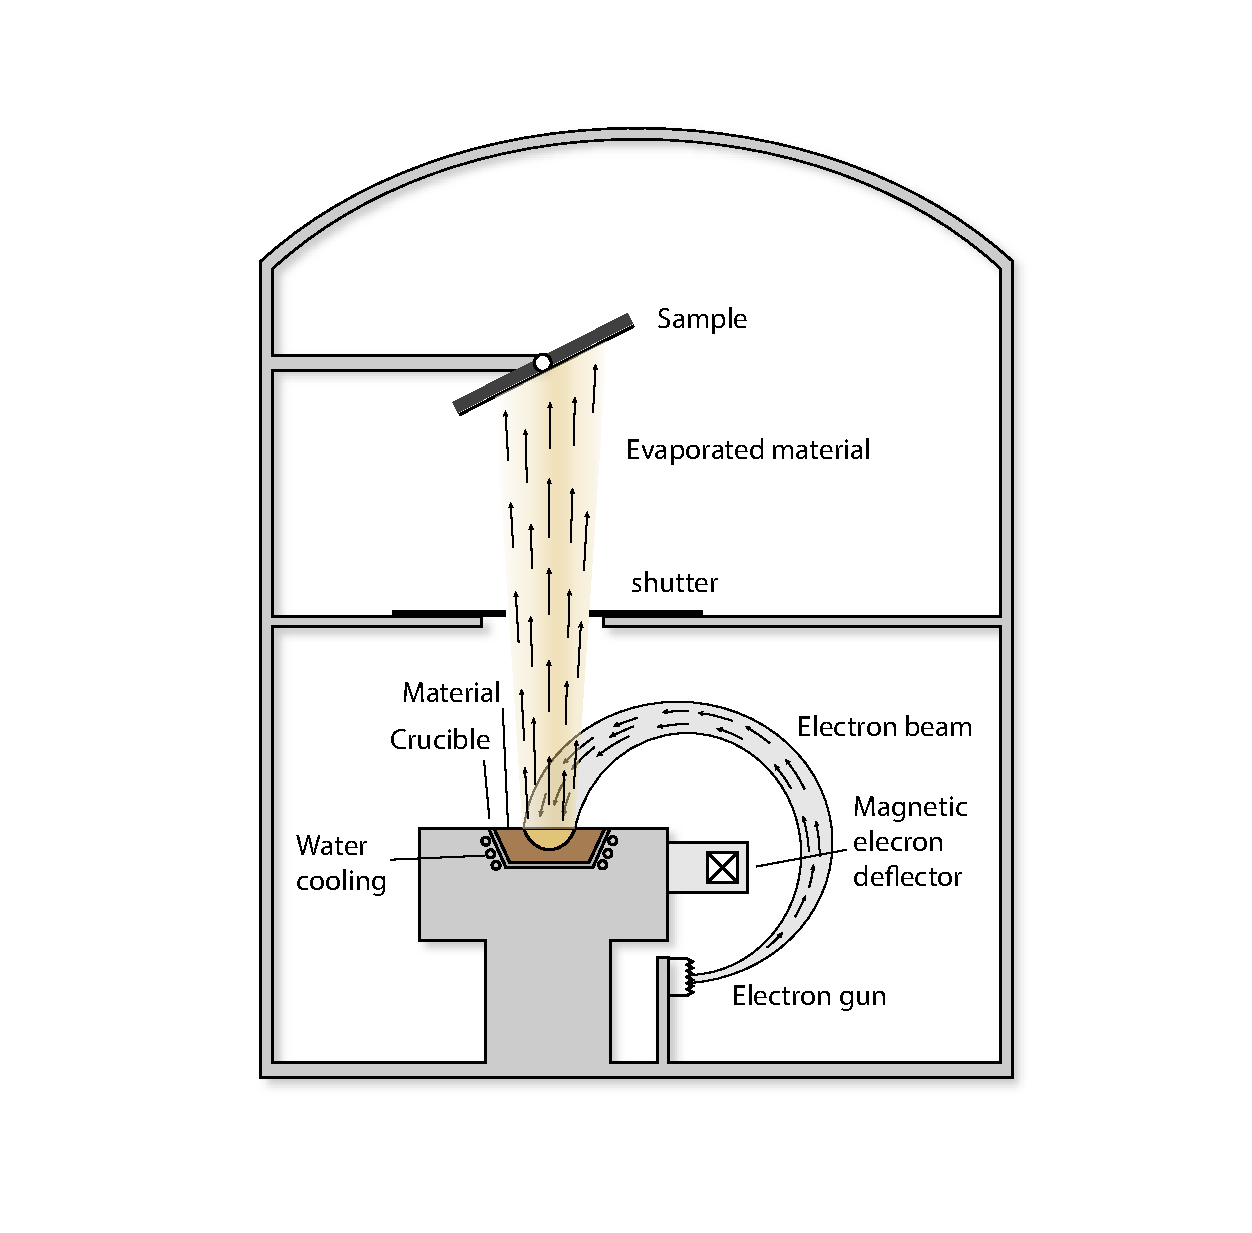
\includegraphics[width=1.0\textwidth]{Drawing/Ebeam.pdf}
	\caption{E-beam evaporator. The electron beam is generated from an electron gun on the bottom. The beam is deviated and shaped by magnetic field, towards the material. Them material is loaded in a crucible and heated up to melting point. The vapor of the material is thrown towards the sample on top. Deposition time is controlled by a shutter.}
	\label{FIG:Ebeam}
\end{figure}

\subsection{Lift-off}

When the sample is patterned with photolithography and coated with metal, the photoresist and the excessive metal need to be removed. Photoresist can dissolve in organic solvents such as acetone. Acetone has high vapor pressure, so it is not suitable to be heated up to increase solubility of photoresist. Also, when acetone dries up on sample it forms streaks. Therefore the sample needs washed with IPA to remove the acetone residue. When the photoresist is heated up to 140 $^{\circ}$C, it will cross-link and its solubility in will decrease. 1165 remover (1-methyl-2-pyrrolidone, or NMP) need to be used for lift-off in such cases. It has low vapor pressure and can be heated up to 80 $^{\circ}$C. If 1165 still cannot fully remove the photoresist after sample is immersed in it for 24 hours, oxygen plasma cleaner is needed.

\subsection{Oxygen plasma cleaning}

The oxygen plasma cleaner activates oxygen molecules with a high frequency voltage (kHz to MHz) in low pressure, and forms plasma or oxygen radicals when electrons recombine with oxygen ions. The mixture is highly reactive and interactive with organic materials like photoresist residue on sample surface. Oxygen plasma cleaning can be categorized as a form of RIE (as discussed in Section \ref{SEC:IonMilling}), but it usually operates at high end of 100 mTorr and the etching is less directional. Compared to chemical solvent, oxygen plasma removes the photoresist residue at a much lower speed (about 10 nm/min), but the finishing is much cleaner, while less invasive compared to RIE. Therefore, oxygen plasma is used as a final step for sample processing.

\section{Graphene/LAO/STO device fabrication}

Current state-of-the-art high quality graphene devices are fabricated from mechanically transferred exfoliated graphene encapsulated with hexagonal boron nitride (h-BN)\cite{dean2010naturenano}, where the mean-free-path of the electron can exceed the dimension of the device\cite{Novoselovaac9439} (tens of micrometers). For applications requiring an arbitrary substrate and graphene shape like my experiment, graphene grown from CVD method and transfer in liquid (``wet-transfer'') is preferred. The basic idea of wet-transfer is to use wet chemical etchant such as nitric acid, hydrochloric acid, FeCl$_3$ or ammonium persulfate (AP) to etch away the metal substrate while the graphene is floating on the liquid surface. The graphene is then scooped out and rinsed in DI-water for several times while floating on water. The substrate is then immersed in the DI-water and used to catch the graphene piece from the bottom. Conventionally, the wet-transfer needs polymers like poly(methyl methacrylate) (PMMA) a scaffold layer to support  graphene on the liquid surface before it is transferred onto the substrate\cite{li2009transfer, reina2008transferring, reina2008large}. The PMMA is then patterned with deep UV exposure or e-beam lithography, so that graphene can be etched in to the designed shape. In the end the PMMA is cleaned with organic solvent. The procedure of using PMMA to transfer and pattern graphene shown in Figure \ref{FIG:PMMATransfer}. 

\begin{figure}[p]
	\centering
	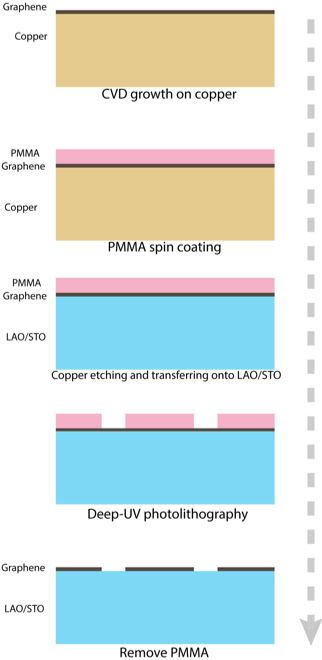
\includegraphics[width=0.450\textwidth]{Drawing/PMMATransfer.png}
	\caption{CVD graphene transfer and patterning with PMMA}
	\label{FIG:PMMATransfer}
\end{figure}

The issue with PMMA as transfer medium is that, the residual PMMA is known to be a source of electron scattering, and would significantly reduce the electron mobilities\cite{pirkle2011effect, lin2011graphene, cheng2011toward}. Annealing the sample in H$_2$/Ar environment proves to partially remove the residue, but the process can also introduce structural defects to graphene\cite{lin2011graphene}, or increase coupling between graphene and the substrate and result in extrinsic doping and deterioration of mobility\cite{cheng2011toward}. 

\begin{figure}[h!]
	\centering
	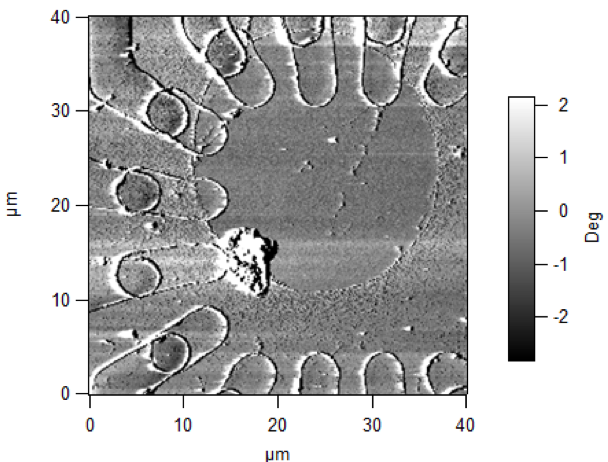
\includegraphics[width=0.60\textwidth]{Drawing/PMMAResidue.png}
	\caption{AFM phase image of graphene on LAO/STO, transferred with PMMA. The circular region is graphene. Particles can be seen outside graphene, on LAO/STO surface.}
	\label{FIG:PMMAResidue}
\end{figure}

Another drawback of using PMMA as a transfer medium is that LAO/STO substrate is susceptible to PMMA contaminants. Figure \ref{} shows the AFM AC phase image of  LAO/STO with a graphene piece transferred and patterned with PMMA. The inside the circular region is graphene. On the LAO/STO surface, contamination particles can be seen. Many experiments in my project require tuning the 2D electron gas on the interface of LAO/STO with c-AFM (will be discussed in Section \ref{SEC:AFM}). Most of the LAO/STO samples were found to lost the interface tunability after the graphene transfer with PMMA. 

A replacement we found for PMMA is a type of perfluoropolymer Hyflon from Solvay. Hyflon has been reported to be widely used in membrane applications such as fuel cells, due to the inertness of C-F bonds\cite{arcella2005hyflon, merlo2007membrane, zhang2012recent}. It has also been reported that the Hyflon membrane between graphene and substrates like SiO$_2$ can reduce the extrinsic p-type doping in graphene by preventing water molecule adsorption to the dangling bonds on the substrates\cite{mattevi2012solution}. It means that, unlike PMMA that leaves residue and deteriorate graphene quality, Hyflon can actually preserve the graphene while used as a transfer medium. Hyflon is also high selectivity to solvent. Most of the organic or inorganic solvent such as acetone, IPA or DI-water cannot dissolve Hyflon, which makes it a perfect protection layer for graphene. 

\subsection{Graphene transfer with Hyflon}

Hyflon is only soluble in perfluorinated solvent. The commercially available Hyflon is in power form. It needs to be dissolved before spin-coated on sample surface. In my experiment I used FC-40 as the solvent. There are different types of Hyflon available, Hyflon AD 40 and Hyflon AD 60, with different molecular weights and phase transition temperature. I have tested both types, and found that graphene transferred with Hyflon AD 60 has higher quality. Although AD 40 has smaller molecular weight, but phase transition temperature might be lower than the soft baking temperature the sample is exposed in processing. This make it hard to remove and affects graphene quality as a result. 


\subsection{Patterning graphene on LAO/STO}

\section{Atomic force microscope}
\label{SEC:AFM}

The atomic force microscope (AFM) is a type of of instrument that uses a nanoscale probe to interact with the surface, and characterize the properties (topography, coulomb interaction, conductivity, etc) of a sample. It was invented in IBM lab by Bin, Quate and Gerber \ref{} in 1986 and later commercialized in 1989. The development of AFM technology benefited from the advancement of STM and precise closed-loop spatial control using piezoelectric effect. However, AFM was invented to overcome the drawback of STM --- only conductive or semi-conductive samples can be measured. AFM can measure various types of interaction between the probe and surface, such as surface potential, magnetic force, Van de Waals force, etc. Also, unlike the scanning electron microscopy (SEM) or tunneling electron microscopy (TEM), the AFM can be operated in various environment (aqueous, ambient, vacuum or cryogenic), and does not require the sample to be pre-treated (such as metal coating) or being conductive. The robustness and non-invasive nature of AFM make it a powerful tool for studying surface phenomena including charge density, magnetic dipole moment, capacitance, chemical bonding, nano-device lithography, and even biomacromolecules. AFM can also be integrated with other techniques, such as infrared spectroscopy\cite{}. The limitation of AFM is that the imaging cannot be as fast as SEM or or TEM, as it relies on the physical movement of the tip.

\subsection{Working principle}


The AFM is mainly consist of three parts, as shown in Figure \ref{FIG:AFM}, AFM tip, laser optics, and piezoelectric scanning system. The AFM tip has a sharp end, with a radius of curvature in nanometer scale. A laser is reflected from the top surface the AFM tip and collected by a quad detector. The quad detector determines the position by
\begin{equation}
\begin{split}
I_\mathrm{sum} & = I_A + I_B + I_C + I_D \\ 
I_\mathrm{vdiff} & = (I_A + I_B) - (I_C + I_D) \\ 
I_\mathrm{hdiff} & = (I_A + I_C) - (I_B + I_D),
\end{split}
\end{equation}
where $I_A$, $I_B$, $I_C$ and $I_D$ are the intensities on the four quadrants of the detector. $I_\mathrm{sum}$ is the total intensity. $I_\mathrm{hdiff}$ and $I_\mathrm{vdiff}$ are the horizontal difference and vertical intensity difference. Assume the laser spot has Gaussian distribution. When the center of laser spot changes, the distribution of intensity on the four quadrant would change. The detector can monitor the movement by the horizontal and vertical differences in intensities. 

\begin{figure}[h!]
	\centering
	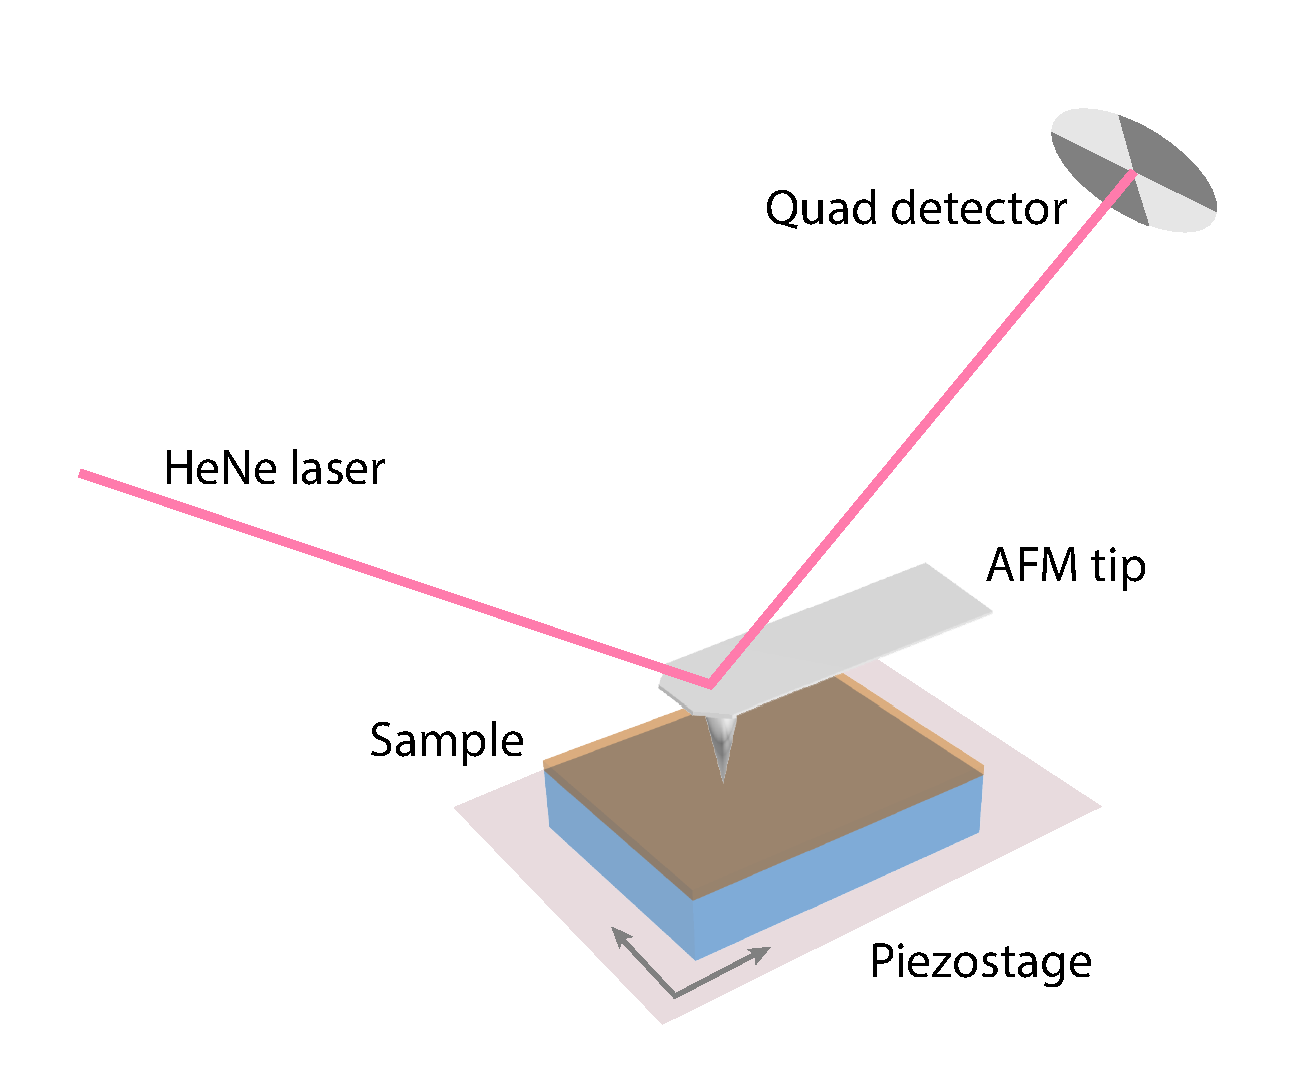
\includegraphics[width=0.8\textwidth]{Drawing/AFM.pdf}
	\caption{The schematics of AFM. A laser is reflected from the top surface of the AFM tip, and collected by a quad detector. A small amount of deformation would cause the center of laser spot to move on the quad detector, and measured as a change of differential voltage.}
	\label{FIG:AFM}
\end{figure}

When the interaction between the tip and sample surface changes and the tip is is slightly deformed, the laser spot would move on the quad detector. The deformation of tip follows Hooke's law:
$$F = -k \cdot x$$
Where $x$ is the amount deformation, and $k$ is the spring constant of the tip cantilever. $k$ is mostly between 1 N/m and 100 N/m, depends on the type of the tip. In my experiment I use tips with spring constant $k = 3$ N/m. The interaction between the AFM tip and sample surface is a function of distance. The attractive interaction decays slower than the repulsive interaction, therefore the total interaction follows the curve in Figure \ref{FIG:Interaction}.

\begin{figure}[h!]
	\centering
	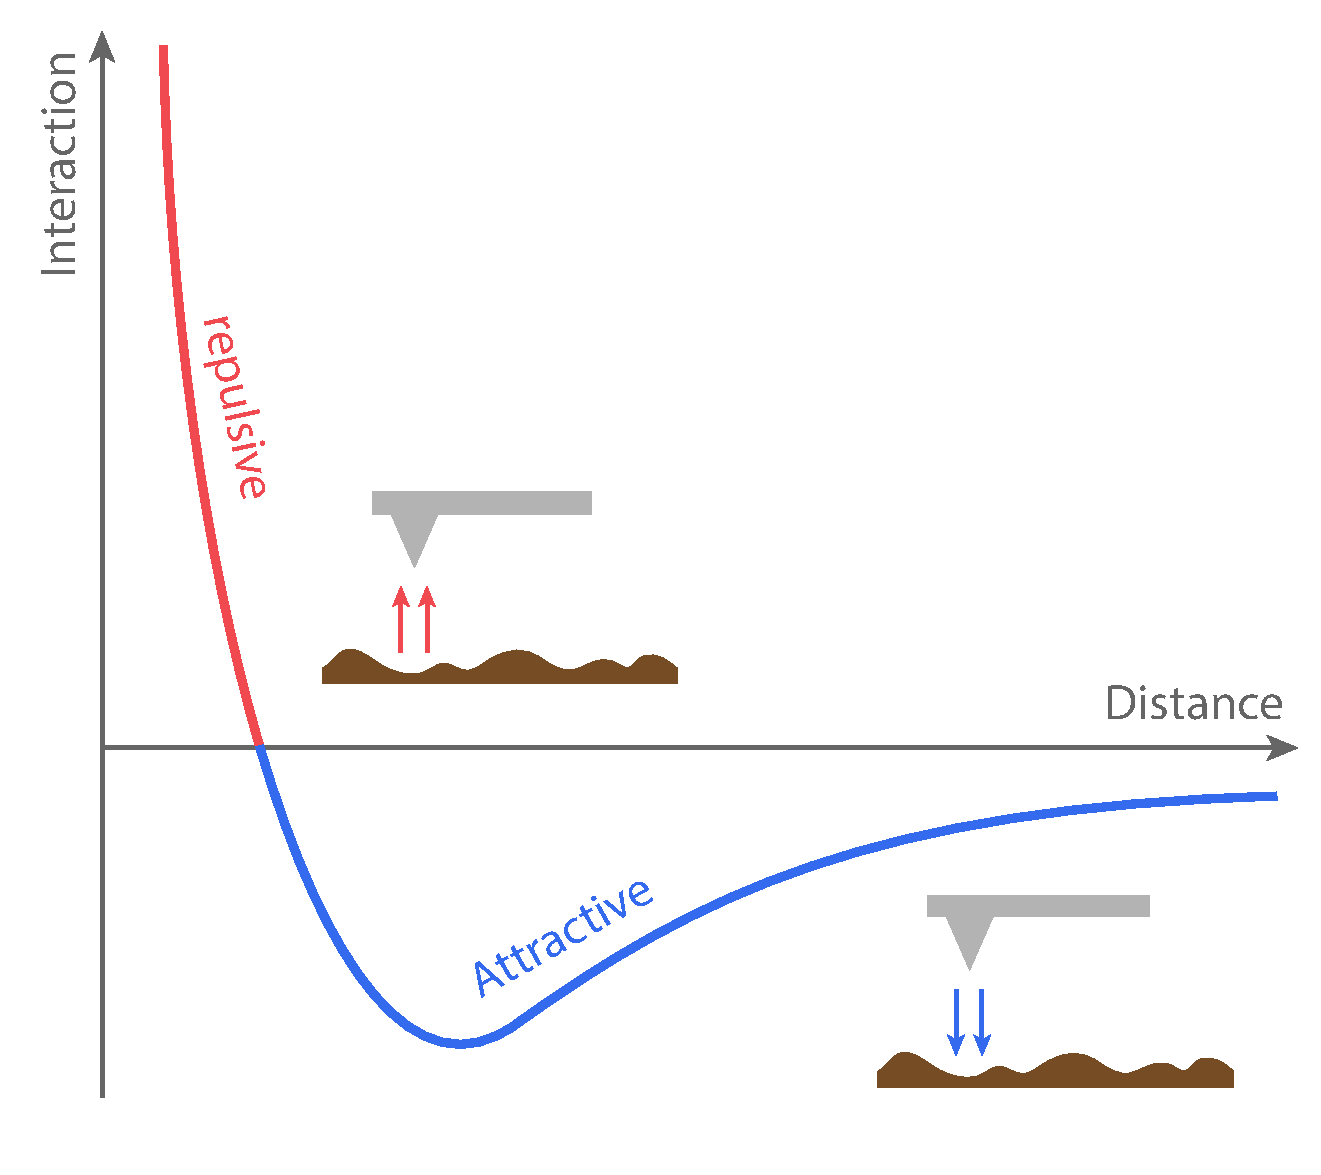
\includegraphics[width=0.7\textwidth]{Drawing/Interaction.pdf}
	\caption{The interaction between tip and the sample surface. At long distance the interaction zero. When the tip moves towards the sample, the interaction is attractive. As the tip gets closer, the interaction would switch from attraction to repulsion, and gets larger and larger the tip moves closer.}
	\label{FIG:Interaction}
\end{figure}

The sample is located on the piezoelectric scanning stage. The movement of the sample and the tip, and signal from the laser optics system are controlled and monitored by a computer. The type of signal depends on the working mode of AFM and nature of the interaction it is targeting. More details are discussed in the following sections. 

\subsection{Contact mode}

In contact mode, the AFM tip is in close contact with the sample. The distance between the tip and sample is controlled by a piezoelectric actuator. As shown in Figure \ref{FIG:ContactAFM}, When the tip approaches the sample surface, repulsion from the sample would deforms the tip and changes the reflection angle of laser spot. The intensity difference on the quad detector would also change, in terms of a voltage signal. When the sample is driven by the piezostage and cause the tip moves relative to the sample, the repulsive force between the tip and sample surface is regulated by a feedback loop between voltage on the piezoelectric actuator, and the voltage difference on the quad detector, so that the amount of tip deformation and repulsive force is a constant. 

\begin{figure}[h!]
	\centering
	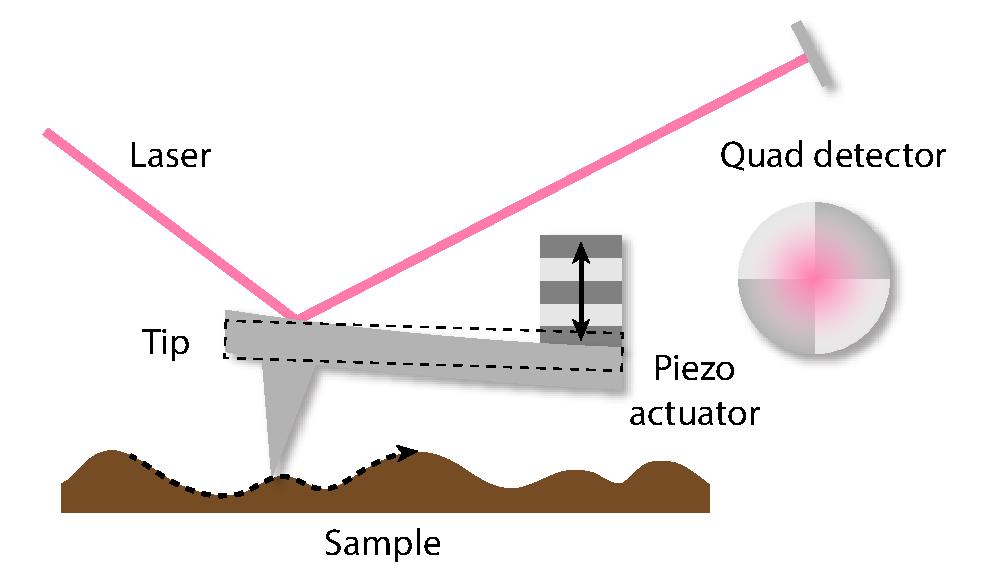
\includegraphics[width=0.6\textwidth]{Drawing/ContactAFM.pdf}
	\caption{AFM contact mode. The tip is pressed to the sample surface by the piezoelectric actuator. The deformation of the tip is monitored by the quad detector. The voltage of the piezoelectric actuator is controlled with a feedback loop with the deflection voltage on the quad detector.}
	\label{FIG:ContactAFM}
\end{figure}


\subsection{AC mode}

In AC mode, the AFM tip is driven by a sinusoidal electrical signal on the tip piezoelectric actuator, as shown in Figure \ref{FIG:ACAFM}. The electric frequency is close to the resonance frequency of the tip (10 kHz - 500 kHz). The driving frequency is not exactly at the resonance frequency, so that the gradient of amplitude change is maximized and the system is most sensitive to the interaction change. The laser spot and difference signal also oscillates at the same frequency. When the tip approaches the sample surface, the interaction between the tip and surface will cause the resonance frequency to shift and change the amplitude $A$ and phase $\theta$ of the tip oscillation and monitored by the differential voltage signal on the quad detector. The measurement can be integrated with lock-in amplifier technique (more discussion can be seen in section \ref{}) for noise reduction. When the tip scan through the surface, $A$ and $\theta$ are recorded for each position on the sample surface and mapped onto a 2D image. The voltage on the piezoelectric actuator ($z$ voltage) is controlled by a feedback loop so that the amplitude $A$ is maintained at a set point. During the scan the tip is not continuously in contact with the sample surface, but ``tapping'' the sample with oscillations, therefore AC mode is sometimes called ``tapping mode''. Compared to contact mode, in the AC mode the tip does not scratch the sample surface, so it has less effect on the sample. 

\begin{figure}[h!]
	\centering
	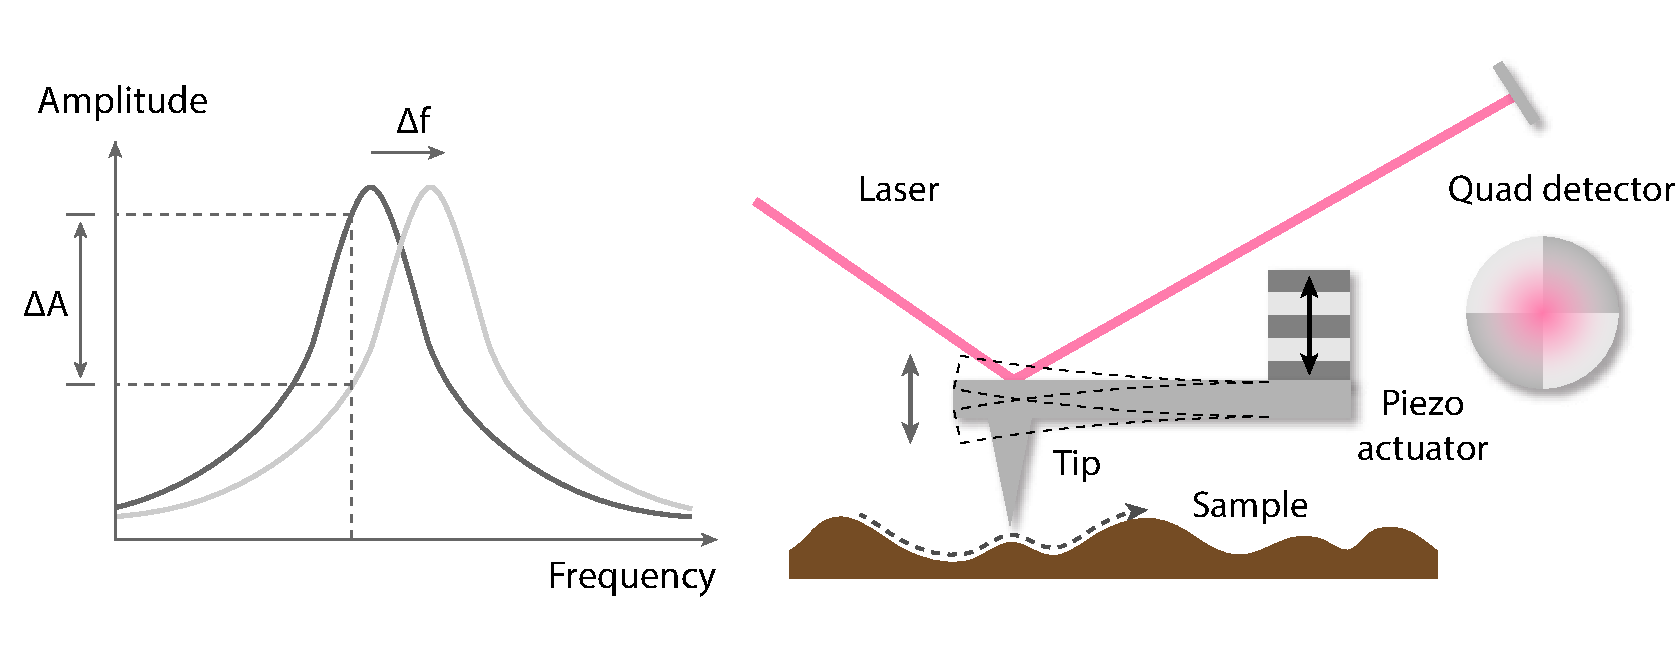
\includegraphics[width=1.0\textwidth]{Drawing/ACAFM.pdf}
	\caption{AFM AC mode. Left: the tip is driven at a frequency close to the resonance frequency. When the resonance frequency shifts as the interaction between the tip and the sample changes, the Change of oscillation amplitude is monitored by the quad detector and sent to the computer.}
	\label{FIG:ACAFM}
\end{figure}

\subsection{Non-contact mode}

In the non-contact mode, the tip is maintained at the attractive regime so that the sample does not have direct contact with the tip. The tip and the sample is maintained at distance that the interaction is always attractive while the tip is scanning through the sample (Figure \ref{FIG:NonContactAFM}). This is especially important for biomacromolecules and organism. 

\begin{figure}[h!]
	\centering
	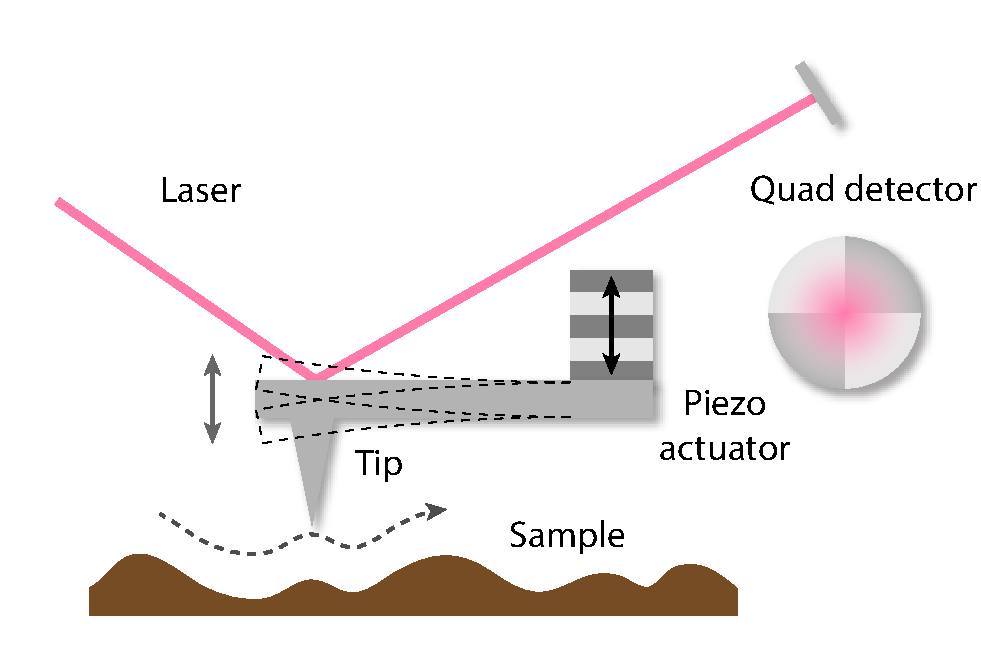
\includegraphics[width=0.6\textwidth]{Drawing/NonContactAFM.pdf}
	\caption{AFM Contact mode. The tip is kept at a distance from the sample so that the interaction is always attractive. The tip does not have direct contact with the sample during the scanning.}
	\label{FIG:NonContactAFM}
\end{figure}

\subsection{Magnetic force microscopy}

When the tip is coated with ferromagnetic materials (e.g. Co, Fe), the AFM is able to measure the magnetic interaction with magnetic force microscopy (MFM). Similar to AC mode, the tip is driven by an oscillating AC voltage close to the resonance frequency (about 100 kHz in my experiments), and the change of interaction is monitored by the amplitude $A$ and phase $\theta$ of the differential voltage on quad detector. The challenge of MFM is that the magnetic and Van der Waals interactions are coupled together. The two-pass technique is used to solve this problem, considering that Van der Waals interaction is short-ranged and decays much faster than the magnetic interaction. First, the tip scans the sample close to the surface, and measures the topography. Second, the tip is lifted and maintained at a constant distance (such as 50 nm) from the sample surface using the height information obtained from the previous scan, so that the Van der Waals interaction is negligible, and the spatial gradient of magnetic force can be measured\cite{hartmann1999magnetic}:
\begin{equation}
%\begin{split}
\label{EQN:MFM}
\Delta A \approx \frac{2 A_0 Q}{3\sqrt{3k}} \cdot \frac{\partial F_z}{\partial z}, \ \ \ \
\Delta \phi \approx \frac{Q}{k} \cdot \frac{\partial F_z}{\partial z}, \ \ \ \
\Delta f \approx -\frac{f_0}{2k} \cdot \frac{\partial F_z}{\partial z}, 
%\end{split}
\end{equation}
where $\Delta A$, $\Delta \phi$ and $\Delta f$ are the change of amplitude, phase and resonance frequency; $A_0$ and $f_0$ are the original amplitude and frequency; $Q$ and k are the resonance quality factor and cantilever spring constant. $\partial F_z/\partial z$ is the spatial gradient of magnetic force. 

Like contact and AC mode of AFM, the resolution of MFM is limited by the tip radius of curvature. Ferromagnetic coating of the MFM tip is about 40 nm in my experiments, so the resolution is in the same order of magnitude. 

The advantage of MFM is that, the resolution and sensitivity is higher than other methods such as magneto-optical effect imaging. Also, like contact and AC mode AFM imaging, MFM does not require special treatment on the sample. The downside of MFM is that the imaging speed is limited by the raster scanning speed. The two-pass method takes twice as long as usual AFM AC scanning. Also, as equation (\ref{EQN:MFM}) shows, MFM signal is not determined by the absolute value of magnetic force, but is proportional to the spatial gradient of the force $\partial F_z/\partial z$, therefore the scanning speed would also affecting the signal. The field from the AFM tip can also affect the magnetic dipoles on the sample, and MFM image can change after each scan. Other long range interaction such as coulomb interaction cannot be eliminated by the two-pass method, and need to be taken care of. More details are discussed in the next chapter. In spite of these disadvantages, the MFM is still a power tool to study surface magnetism for its robustness and simplicity of operations.

\begin{figure}[h!]
	\centering
	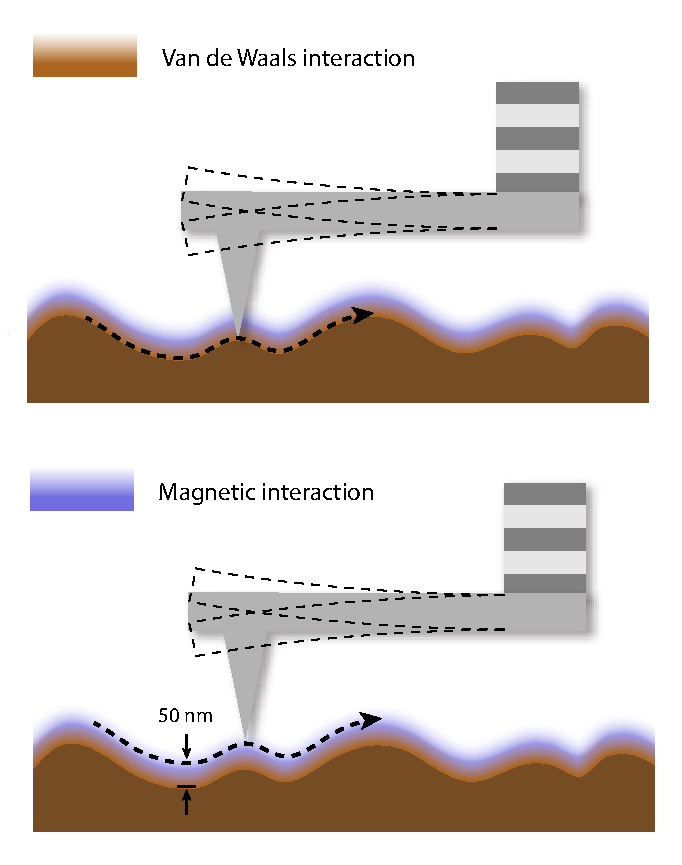
\includegraphics[width=0.5\textwidth]{Drawing/MFM.pdf}
	\caption{MFM mode. The first scan is close to the sample surface, so that the topographical information can be obtained. In the second scan the tip is lifted to a constant distance from the sample surface, so that the Van der Waals interaction is negligible and only the long-ranged magnetic interaction is measured.}
	\label{FIG:MFM}
\end{figure}

\subsection{Piezoresponse force microscopy}

The high sensitivity and extendability of AFM make it a versatile tool to measure different types of interactions between the tip and sample. One important variant is piezoresonse force microscopy (PFM). Piezoelectric effect is the phenomenon when an external stress or strain is applied to a piezoelectric material, the deformation will induce electric dipole moments and build up an internal electric potential across the sample. Inversely, the external electric field can also induce mechanical deformation. Depending on the properties of the material, the deformation can be either expansion or contraction. The effect can be described with
$$
X_i = d_{ki}E_k,
$$
where $X_i$ is the strain tensor, $d_{ki}$ is the piezoelectric tensor and $E_k$ is the electric field. For a tetragonal system, 
$$
\begin{bmatrix}
	X_{1} \\
	X_{2} \\
	X_{3} \\
	X_{4} \\
	X_{5} \\
	X_{6}
\end{bmatrix} =
\begin{bmatrix}
	0 & 0 & d_{31} \\
	0 & 0 & d_{32} \\
	0 & 0 & d_{33} \\
	0 & d_{15} & 0 \\
	d_{15} & 0 & 0 \\
	0 & 0 & 0
\end{bmatrix}
\begin{bmatrix}
	E_{1} \\
	E_{2} \\
	E_{3}
\end{bmatrix}
$$
When a field is applied in $E_3$ direction, the resulting non-zero strain terms are $X_1 = d_{31}E_3$, $X_2 = d_{32}E_3$ and $X_3 = d_{33}E3$. Therefore, an electric field in the c-axis of the crystal will cause elongation in the c-axis and contraction in the other two orthogonal directions, or vice versa. The piezoresponse of sample can bring insights of the sample properties such as carrier concentration\cite{}, ferroelectric domain orientation\cite{}, domain boundary\cite{}, etc.

In PFM measurement, a conductive tip made of doped silicon or coated with metal is in contact with the sample and a sinusoidal voltage signal is applied to the tip. For a sample with piezoresponse, the electric field will cause a deformation of the sample topography sinusoidal in time. Since the sample is in contact with the tip, the topographical change of sample will cause slight change of tip deformation and the change is recorded by the differential voltage on the quad detector. The sample deformation is usually in the order of 10 pm/V (e.g. 85.6 pm/V for BaTiO$_3$\cite{}). Therefore, PFM signal is measured with lock-in technique for the best signal-to-noise ratio. As shown in Figure \ref{FIG:PFM}, If the sample contract in the direction of the electric field, the piezoresponse signal will be in phase with the electric signal; if the sample elongate in the direction of the field, the signal will be out of phase.

\begin{figure}[h!]
	\centering
	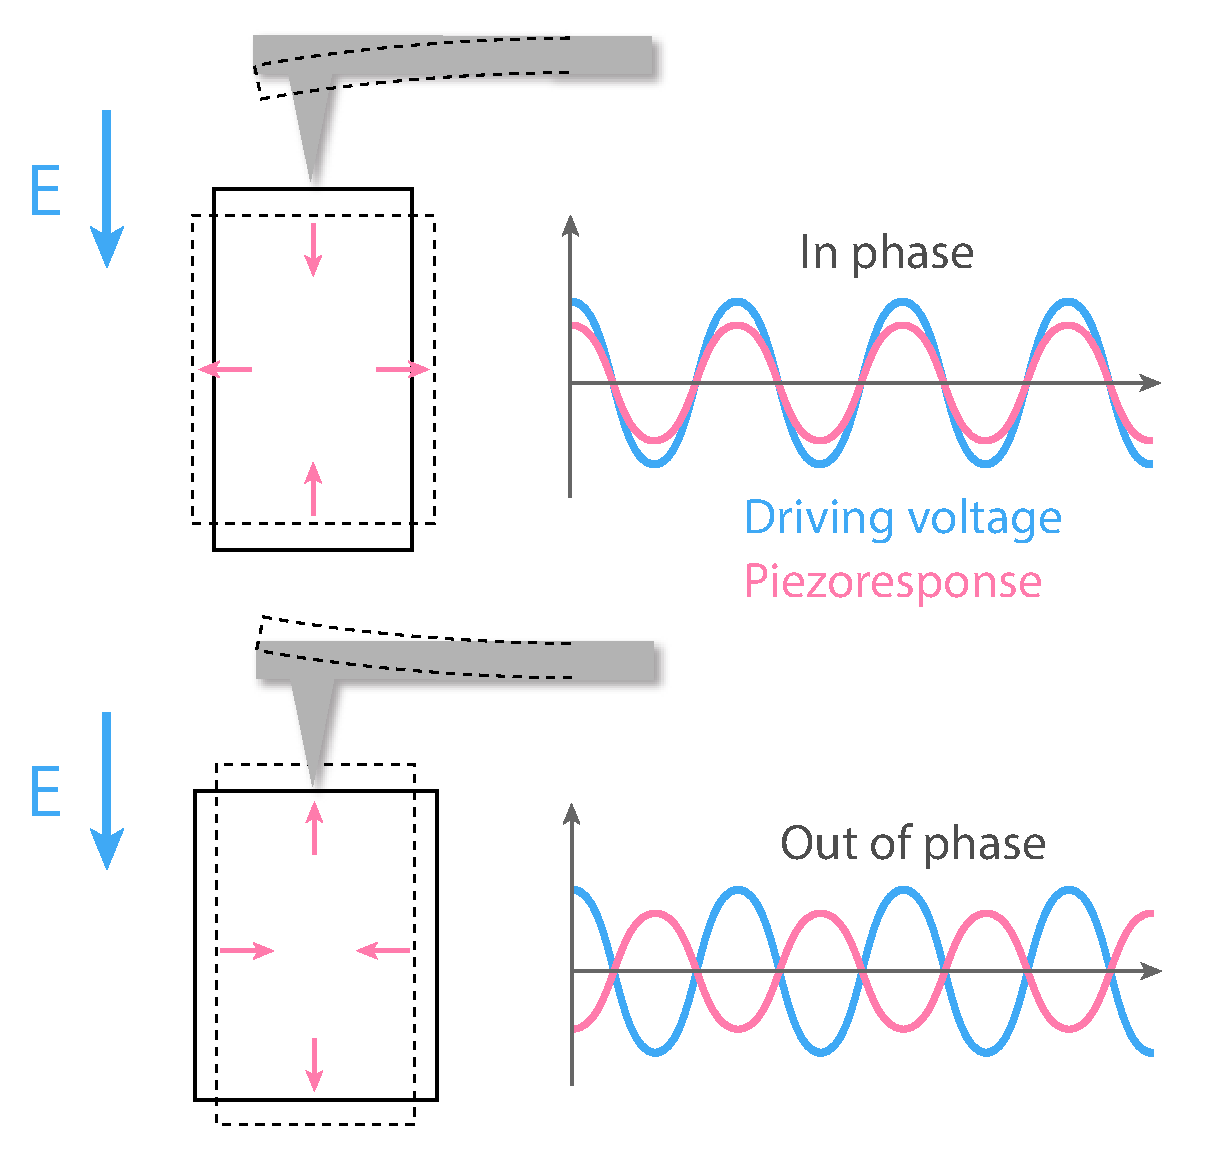
\includegraphics[width=0.7\textwidth]{Drawing/PFM.pdf}
	\caption{PFM measurement. The external electric field is applied on the sample through a conductive tip. The sample deforms and slightly bend the tip, and the deformation signal is monitored with a quad detector (not shown). If the sample contract in the direction of the field, the deformation signal is in phase with the driving voltage (above); if the sample elongate in the direction of the field, the signal would be out of phase with the driving voltage (below).}
	\label{FIG:PFM}
\end{figure}

\subsection{LAO/STO nano-device c-AFM lithography}

\subsection{Graphene/LAO/STO nano-device lithography}

\section{Electronic signal measurement}

\chapter{Graphene p-n junction edge-state engineering}

\chapter{Graphene/LAO/STO superlattice device}

\chapter{Magneto-Optical Kerr Effect on LAO/STO interface}

\section{Motivation}

\section{Experimental setup}

\section{Results}

\chapter{Outlook}
	
\chapter{Conclusions}


%
%\appendix                          % After this command, chapters will be formatted as appendices. For example:

%
\safebibliography{main}          %\safebibliography is used the same way as \bibliography, but gives pittetd
%                                   a greater chance to succeed in formatting the bibliography when non-standard
% 

                                  %BibTeX styles are used.
\end{document}
